%% abtex2-modelo-trabalho-academico.tex, v-1.9.7 laurocesar
%% Copyright 2012-2018 by abnTeX2 group at http://www.abntex.net.br/ 
%%
%% This work may be distributed and/or modified under the
%% conditions of the LaTeX Project Public License, either version 1.3
%% of this license or (at your option) any later version.
%% The latest version of this license is in
%%   http://www.latex-project.org/lppl.txt
%% and version 1.3 or later is part of all distributions of LaTeX
%% version 2005/12/01 or later.
%%
%% This work has the LPPL maintenance status `maintained'.
%% 
%% The Current Maintainer of this work is the abnTeX2 team, led
%% by Lauro César Araujo. Further information are available on 
%% http://www.abntex.net.br/
%%
%% This work consists of the files abntex2-modelo-trabalho-academico.tex,
%% abntex2-modelo-include-comandos and abntex2-modelo-references.bib
%%

% ------------------------------------------------------------------------
% ------------------------------------------------------------------------
% abnTeX2: Modelo de Trabalho Academico (tese de doutorado, dissertacao de
% mestrado e trabalhos monograficos em geral) em conformidade com 
% ABNT NBR 14724:2011: Informacao e documentacao - Trabalhos academicos -
% Apresentacao
% ------------------------------------------------------------------------
% ------------------------------------------------------------------------

\documentclass[
	% -- opções da classe memoir --
	12pt,						% tamanho da fonte
	openright,					% capítulos começam em pág ímpar (insere página vazia caso preciso)
	oneside,					% para impressão em recto e verso. Oposto a oneside
	a4paper,					% tamanho do papel. 
	% -- opções da classe abntex2 --
	%chapter=TITLE,				% títulos de capítulos convertidos em letras maiúsculas
	%section=TITLE,				% títulos de seções convertidos em letras maiúsculas
	%subsection=TITLE,			% títulos de subseções convertidos em letras maiúsculas
	%subsubsection=TITLE,		% títulos de subsubseções convertidos em letras maiúsculas
	% -- opções do pacote babel --
	english,					% idioma adicional para hifenização
	french,						% idioma adicional para hifenização
	spanish,					% idioma adicional para hifenização
	brazil						% o último idioma é o principal do documento
	]{abntex2}


\usepackage{lmodern}			% Usa a fonte Latin Modern			
\usepackage[T1]{fontenc}		% Selecao de codigos de fonte.
\usepackage[utf8]{inputenc}		% Codificacao do documento (conversão automática dos acentos)
\usepackage{indentfirst}		% Indenta o primeiro parágrafo de cada seção.
\usepackage{color}				% Controle das cores
\usepackage{graphicx}			% Inclusão de gráficos
\usepackage{microtype} 			% para melhorias de justificação
\usepackage{lipsum}				% para geração de dummy text
\usepackage[brazilian,hyperpageref]{backref}	 % Paginas com as citações na bibl
\usepackage[alf]{abntex2cite}	% Citações padrão ABNT
\usepackage{multirow}

\usepackage{forest}
\usepackage{fontawesome}

\definecolor{thered}{rgb}{0.65,0.04,0.07}
\definecolor{thegreen}{rgb}{0.06,0.44,0.08}
\definecolor{thegrey}{gray}{0.5}
\definecolor{theshade}{rgb}{1,1,0.97}
\definecolor{theframe}{gray}{0.6}
\definecolor{blue}{RGB}{41,5,195} 

\usepackage{listings}
\lstset{
	basicstyle=\small, % print whole listing small
	keywordstyle=\color{blue}\bfseries, %\underbar,% underlined bold black keywords
	% keywords=[0]{uint32_t, exit},
	% keywordstyle=[0]\color{thered},
	identifierstyle=, % nothing happens
	commentstyle=\color{gray!85}, % white comments
	stringstyle=\color{thered}\ttfamily, % typewriter type for strings
	showstringspaces=false, % no special string spaces
	numbers=left,
	numberstyle=\tiny,
	stepnumber=2
}

\definecolor{folderbg}{RGB}{124,166,198}
\definecolor{folderborder}{RGB}{110,144,169}

\def\Size{4pt}
\tikzset{
  folder/.pic={
    \filldraw[draw=folderborder,top color=folderbg!50,bottom color=folderbg]
      (-1.05*\Size,0.2\Size+5pt) rectangle ++ (.75*\Size,-0.2\Size-5pt);  
    \filldraw[draw=folderborder,top color=folderbg!50,bottom color=folderbg]
      (-1.15*\Size,-\Size) rectangle (1.15*\Size,\Size);
  }
}


% Configurações do pacote backref
% Usado sem a opção hyperpageref de backref
\renewcommand{\backrefpagesname}{Citado na (s) página (s):~}
% Texto padrão antes do número das páginas
\renewcommand{\backref}{}
% Define os textos da citação
\renewcommand*{\backrefalt}[4]{
	\ifcase#1
		Nenhuma citação no texto.%
	\or%
		Citado na página #2.%
	\else
		Citado #1 vezes nas páginas #2.%
	\fi}%


%-------------------------------------------------------------------------------------
%		DADOS PESSOAIS
%		Informações básicas sobre os trabalho e os autores 
%-------------------------------------------------------------------------------------
\titulo{Desenvolvimento de um co-processador de vídeo em FPGA para integração com o Robot Operating System - ROS}
\autor{Nestor Dias Pereira Neto}
\local{Salvador}
\data{Outubro 2022}
\orientador{Wagner Luiz Alves de Oliveira}
\coorientador{Paulo César Machado de Abreu Farias}
\tipotrabalho{Dissertação (Mestrado)} 
\preambulo{Esta Dissertação de Mestrado foi apresentada ao Programa de Pós Graduação em Engenharia Elétrica da Universidade Federal da Bahia, como requisito parcial para obtenção do grau de Mestre em Engenharia Elétrica.}

\instituicao{%
  Universidade Federal da Bahia - UFBA
  \par
  Escola Politécnica
  \par
  Programa de Pós-Graduação em Engenharia Elétrica}


%	Configurações de aparência do PDF final
% alterando o aspecto da cor azul
\definecolor{blue}{RGB}{41,5,195}

% informações do PDF
\makeatletter
\hypersetup{
     	%pagebackref=true,
		pdftitle={\@title}, 
		pdfauthor={\@author},
    	pdfsubject={\imprimirpreambulo},
	    pdfcreator={LaTeX with abnTeX2},
		pdfkeywords={abnt}{latex}{abntex}{abntex2}{trabalho acadêmico}, 
		colorlinks=true,       		% false: boxed links; true: colored links
    	linkcolor=blue,          	% color of internal links
    	citecolor=blue,        		% color of links to bibliography
    	filecolor=magenta,      		% color of file links
		urlcolor=blue,
		bookmarksdepth=4
}
\makeatother


% Posiciona figuras e tabelas no topo da página quando adicionadas sozinhas em um página em branco. 
% Ver https://github.com/abntex/abntex2/issues/170
\makeatletter
\setlength{\@fptop}{5pt} % Set distance from top of page to first float
\makeatother

% Possibilita criação de Quadros e Lista de quadros. Ver https://github.com/abntex/abntex2/issues/176
\newcommand{\quadroname}{Quadro}
\newcommand{\listofquadrosname}{Lista de quadros}

\newfloat[chapter]{quadro}{loq}{\quadroname}
\newlistof{listofquadros}{loq}{\listofquadrosname}
\newlistentry{quadro}{loq}{0}

% configurações para atender às regras da ABNT
\setfloatadjustment{quadro}{\centering}
\counterwithout{quadro}{chapter}
\renewcommand{\cftquadroname}{\quadroname\space} 
\renewcommand*{\cftquadroaftersnum}{\hfill--\hfill}

\setfloatlocations{quadro}{hbtp}

% O tamanho do parágrafo é dado por:
\setlength{\parindent}{1.3cm}

% Controle do espaçamento entre um parágrafo e outro:
\setlength{\parskip}{0.2cm}  % tente também \onelineskip


\makeindex





%%%%%%%%%%%%%%%%%%%%%%%%%%%%%%%%%%%%%%%%%%%%%%%%%%%%%%%%%%%%%%%%%%%%%%%%%%%%%%%%%%%%%%
%																					 %
% 							 Início do documento								     %
%																					 %
%%%%%%%%%%%%%%%%%%%%%%%%%%%%%%%%%%%%%%%%%%%%%%%%%%%%%%%%%%%%%%%%%%%%%%%%%%%%%%%%%%%%%%
\begin{document}

%\selectlanguage{english}
\selectlanguage{brazil}

% Retira espaço extra obsoleto entre as frases.
\frenchspacing 

%-------------------------------------------------------------------------------------
% 		ELEMENTOS PRÉ-TEXTUAIS
%		Insire elementos pré textuais, ficha catalográfica 
%-------------------------------------------------------------------------------------
% \pretextual

\imprimircapa\imprimirfolhaderosto*	% (o * indica que haverá a ficha bibliográfica)

% Isto é um exemplo de Ficha Catalográfica, ou ``Dados internacionais de
% catalogação-na-publicação''. Você pode utilizar este modelo como referência. 
% Porém, provavelmente a biblioteca da sua universidade lhe fornecerá um PDF
% com a ficha catalográfica definitiva após a defesa do trabalho. Quando estiver
% com o documento, salve-o como PDF no diretório do seu projeto e substitua todo
% o conteúdo de implementação deste arquivo pelo comando abaixo:
%
% \begin{fichacatalografica}
%     \includepdf{fig_ficha_catalografica.pdf}
% \end{fichacatalografica}
\begin{fichacatalografica}
	\sffamily
	\vspace*{\fill}					% Posição vertical
	\begin{center}					% Minipage Centralizado
	\fbox{\begin{minipage}[c][8cm]{13.5cm}		% Largura
	\small
	\imprimirautor
	%Sobrenome, Nome do autor
	
	\hspace{0.5cm} \imprimirtitulo  / \imprimirautor. --
	\imprimirlocal, \imprimirdata-
	
	\hspace{0.5cm} \thelastpage p. : il. (algumas color.) ; 30 cm.\\
	
	\hspace{0.5cm} \imprimirorientadorRotulo~\imprimirorientador\\
	
	\hspace{0.5cm}
	\parbox[t]{\textwidth}{\imprimirtipotrabalho~--~\imprimirinstituicao,
	\imprimirdata.}\\
	
	\hspace{0.5cm}
		1. Palavra-chave1.
		2. Palavra-chave2.
		2. Palavra-chave3.
		I. Orientador.
		II. Universidade xxx.
		III. Faculdade de xxx.
		IV. Título 			
	\end{minipage}}
	\end{center}
\end{fichacatalografica}
%---
%
\begin{errata}
Elemento opcional da \citeonline[4.2.1.2]{NBR14724:2011}. Exemplo:

\vspace{\onelineskip}

FERRIGNO, C. R. A. \textbf{Tratamento de neoplasias ósseas apendiculares com
reimplantação de enxerto ósseo autólogo autoclavado associado ao plasma
rico em plaquetas}: estudo crítico na cirurgia de preservação de membro em
cães. 2011. 128 f. Tese (Livre-Docência) - Faculdade de Medicina Veterinária e
Zootecnia, Universidade de São Paulo, São Paulo, 2011.

\begin{table}[htb]
\center
\footnotesize
\begin{tabular}{|p{1.4cm}|p{1cm}|p{3cm}|p{3cm}|}
  \hline
   \textbf{Folha} & \textbf{Linha}  & \textbf{Onde se lê}  & \textbf{Leia-se}  \\
    \hline
    1 & 10 & auto-conclavo & autoconclavo\\
   \hline
\end{tabular}
\end{table}

\end{errata}

% ---
% Inserir folha de aprovação
% ---

% Isto é um exemplo de Folha de aprovação, elemento obrigatório da NBR
% 14724/2011 (seção 4.2.1.3). Você pode utilizar este modelo até a aprovação
% do trabalho. Após isso, substitua todo o conteúdo deste arquivo por uma
% imagem da página assinada pela banca com o comando abaixo:
%
% \begin{folhadeaprovacao}
% \includepdf{folhadeaprovacao_final.pdf}
% \end{folhadeaprovacao}
%
\begin{folhadeaprovacao}

  \begin{center}
    {\ABNTEXchapterfont\large\imprimirautor}

    \vspace*{\fill}\vspace*{\fill}
    \begin{center}
      \ABNTEXchapterfont\bfseries\Large\imprimirtitulo
    \end{center}
    \vspace*{\fill}
    
    \hspace{.45\textwidth}
    \begin{minipage}{.5\textwidth}
        \imprimirpreambulo
    \end{minipage}%
    \vspace*{\fill}
   \end{center}
        
   Trabalho aprovado. \imprimirlocal, 24 de novembro de 2012:

   \assinatura{\textbf{\imprimirorientador} \\ Orientador} 
   \assinatura{\textbf{Professor} \\ Convidado 1}
   \assinatura{\textbf{Professor} \\ Convidado 2}
   %\assinatura{\textbf{Professor} \\ Convidado 3}
   %\assinatura{\textbf{Professor} \\ Convidado 4}
      
   \begin{center}
    \vspace*{0.5cm}
    {\large\imprimirlocal}
    \par
    {\large\imprimirdata}
    \vspace*{1cm}
  \end{center}
  
\end{folhadeaprovacao}
% ---
%% ---
% Dedicatória
% ---
\begin{dedicatoria}
   \vspace*{\fill}
   \centering
   \noindent
   \textit{ Este trabalho é dedicado às crianças adultas que,\\
   quando pequenas, sonharam em se tornar cientistas.} \vspace*{\fill}
\end{dedicatoria}
% ---
%% ---
% Agradecimentos
% ---
\begin{agradecimentos}
Os agradecimentos principais são direcionados à Gerald Weber, Miguel Frasson,
Leslie H. Watter, Bruno Parente Lima, Flávio de Vasconcellos Corrêa, Otavio Real
Salvador, Renato Machnievscz\footnote{Os nomes dos integrantes do primeiro
projeto abn\TeX\ foram extraídos de
\url{http://codigolivre.org.br/projects/abntex/}} e todos aqueles que
contribuíram para que a produção de trabalhos acadêmicos conforme
as normas ABNT com \LaTeX\ fosse possível.

Agradecimentos especiais são direcionados ao Centro de Pesquisa em Arquitetura
da Informação\footnote{\url{http://www.cpai.unb.br/}} da Universidade de
Brasília (CPAI), ao grupo de usuários
\emph{latex-br}\footnote{\url{http://groups.google.com/group/latex-br}} e aos
novos voluntários do grupo
\emph{\abnTeX}\footnote{\url{http://groups.google.com/group/abntex2} e
\url{http://www.abntex.net.br/}}~que contribuíram e que ainda
contribuirão para a evolução do \abnTeX.

\end{agradecimentos}
% ---
%
% ---
% Epígrafe
% ---
\begin{epigrafe}
    \vspace*{\fill}
	\begin{flushright}
		\textit{``Não vos amoldeis às estruturas deste mundo, \\
		mas transformai-vos pela renovação da mente, \\
		a fim de distinguir qual é a vontade de Deus: \\
		o que é bom, o que Lhe é agradável, o que é perfeito.\\
		(Bíblia Sagrada, Romanos 12, 2)}
	\end{flushright}
\end{epigrafe}
% ---

% ---
% RESUMOS
% ---

% resumo em português
\setlength{\absparsep}{18pt} % ajusta o espaçamento dos parágrafos do resumo
\begin{resumo}
 Segundo a \citeonline[3.1-3.2]{NBR6028:2003}, o resumo deve ressaltar o
 objetivo, o método, os resultados e as conclusões do documento. A ordem e a extensão
 destes itens dependem do tipo de resumo (informativo ou indicativo) e do
 tratamento que cada item recebe no documento original. O resumo deve ser
 precedido da referência do documento, com exceção do resumo inserido no
 próprio documento. (\ldots) As palavras-chave devem figurar logo abaixo do
 resumo, antecedidas da expressão Palavras-chave:, separadas entre si por
 ponto e finalizadas também por ponto.

 \textbf{Palavras-chave}: latex. abntex. editoração de texto.
\end{resumo}v
% resumo em inglês
\begin{resumo}[Abstract]
 \begin{otherlanguage*}{english}

  The new projects in robotics have demanded more and more processing power, consequently, requiring greater energy efficiency, especially in applications that make use of batteries.
  In this way, the use of the FPGA can contribute to a gain in processing power associated with low consumption. In this work, a method was developed to establish communication between the ROS and an FPGA embedded in a SoC of the Cyclone V family. Through a server-client system, through a Gigabit ethernet link, it was possible to establish communication between the elements of the system. Performance tests were performed on the DE10-Nano development kit and reached a considered acceptable result.


   \vspace{\onelineskip}
 
   \noindent 
   \textbf{Keywords}: ROS, FPGA, SoC, Cyclone V.
 \end{otherlanguage*}
\end{resumo}

% resumo em francês 
%\begin{resumo}[Résumé]
% \begin{otherlanguage*}{french}
%    Il s'agit d'un résumé en français.
% 
%   \textbf{Mots-clés}: latex. abntex. publication de textes.
% \end{otherlanguage*}
%\end{resumo}

% resumo em espanhol
%\begin{resumo}[Resumen]
% \begin{otherlanguage*}{spanish}
%   Este es el resumen en español.
%  
%   \textbf{Palabras clave}: latex. abntex. publicación de textos.
% \end{otherlanguage*}
%\end{resumo}
% ---

%% ---
% inserir lista de ilustrações
% ---
\pdfbookmark[0]{\listfigurename}{lof}
\listoffigures*
\cleardoublepage
% ---

% ---
% inserir lista de quadros
% ---
\pdfbookmark[0]{\listofquadrosname}{loq}
\listofquadros*
\cleardoublepage
% ---

% ---
% inserir lista de tabelas
% ---
\pdfbookmark[0]{\listtablename}{lot}
\listoftables*
\cleardoublepage
% ---
%% ---
% inserir lista de abreviaturas e siglas
% ---
\begin{siglas}
  \item[ABNT] Associação Brasileira de Normas Técnicas
  \item[abnTeX] ABsurdas Normas para TeX
\end{siglas}
% ---
%\include{pre-textuais/listas_simbolos}

% inserir o sumario
\pdfbookmark[0]{\contentsname}{toc}
\tableofcontents*
\cleardoublepage%

%-------------------------------------------------------------------------------------
% 		ELEMENTOS TEXTUAIS
%		Informações relevantes ao trabalho, capítulos e suas respectivas seções.
%-------------------------------------------------------------------------------------
\textual%

\chapter{Introdução}\label{cap:intro}

% Apresentação do Tema e Contexto
% Nesta parte do documento, o pesquisador precisa explicar no texto a respeito do contexto 
% em que o tema está inserido. É bom imaginar que o leitor não conhece da área então 
% antes de explicar o assunto específico que será abordado, você deve explicar onde ele 
% está inserido.

Nos últimos anos novas técnicas para construção de robôs tem estado em muita evidência, em especial áreas como robótica móvel e robótica colaborativa têm chamado bastante atenção dos pesquisadores. Uma das principais características dessas áreas é a exigência de um alto grau de percepção do ambiente que rodeia o robô, além de uma execução mais precisa em seus movimentos, isto devido ao fato de que as atividades desempenhadas por estes robôs estão exigindo um nível cada vez maior de interação com as atividades desempenhadas por seres humanos.

Este grau de precisão requerido no desenvolvimento de novos robôs demandam um poder de processamento cada vez maior, consequentemente, elevando o consumo energético, o que pode vir a ser um problema principalmente em sistemas que fazem uso de baterias. Uma excelente alternativa para adicionar poder de processamento aliado ao baixo consumo é o uso do FPGA\@. O potencial que os FPGAs possuem para melhorar o desempenho de sistemas computacionais já é bem conhecido há algum tempo, as possibilidades de paralelismo e criação de estruturas de DSP dedicadas, são recursos muito interessantes que o hardware configurado oferece. 

Entretanto as facilidades de desenvolvimento encontradas em aplicações que fazem uso de softwares não estão disponíveis na mesma proporção no mundo do hardware configurável. A maio dificuldade no desenvolvimento de soluções que fazem uso do FPGA tornam os seus projetos mais longo, e necessitam de mão de obra extremamente especializada, o que fazem seu desenvolvimento mais caro. Isso faz com que o seu uso em projetos de robótica seja pouco usado e ate mesmo desistimulado. 

Atualmente o \textit{framework} ROS está se consolidando como o padrão na criação de novas plataformas robóticas, tanto no desenvolvimento de manipuladores colaborativos quanto na robótica móvel. O objetivo do ROS é facilitar a elaboração de novos robôs, através de um conjunto completo de ferramentas para desenvolvimento, como \textit{drivers} para sensores e atuadores, bibliotecas e principalmente reuso de código. Agrupar inúmeros ``blocos'' de softwares usados em robótica, fornecer drivers para hardwares específicos (sensores e atuadores), gerenciar troca de mensagens entre os nós que fazem parte do sistema, são as função do ROS\@. 

Estas características fazem com que o ROS seja reconhecido com um pseudo sistema operacional~\cite{rosPYO}. Dessa maneira o ROS se tornou muito ágil no desenvolvimento de novas aplicações para robótica. Usando aplicações já desenvolvidas e testadas por outros desenvolvedores, podemos criar novos sistemas completos apenas gerenciando estas aplicações na estrutura interna do ROS. Essa abordagem fez com que o número de pacotes para o ROS cresça em uma taxa muito rápida, desde o ano de seu lançamento, em 2007, até 2012 o ROS aumentou de 1 para 3699 pacotes~\cite{fpgarobotics}.

Aproveitar as facilidades de desenvolvimento proporcionadas pelo ROS em conjunto com o alto poder de processamento e baixo consumo que o FPGA oferece, seria um cenário ideal no desenvolvimento de novas aplicações com robôs. Para isso, precisamos estabelecer uma conexão com uma taxa de transferência de dados alta o suficiente para não influenciar de forma negativa no tempo de processamento e, que torne relativamente fácil seu uso por desenvolvedores especializados em robótica, mas sem grande experiência em FPGA. Portanto, este trabalho tem como objetivo estabelecer uma comunicação de alto desempenho entre ROS e um FPGA para que se possa aproveitar o melhor das duas tecnologias em projetos de robótica. 

explicar a parte da comunicação entre o computador/ros e o SoC melhorar a comunicação, comunicação eficiente, pacote pronto e de fácil integração com qualquer sistema ros, O mais genérico possível para se enquadrar a qualquer projeto é que o desenvolvedor tenha interesse em incluir um FPGA ao sistema



\begin{itemize}
    \item \textbf{Como estabelecer a comunicação entre o ROS e um sistema de processamento auxiliar 
embarcado em um FPGA?}

\end{itemize}

Este problema é o que o trabalho vai tentar resolver, possibilitando assim, o uso de aceleração por hardware através do fpga, ser incluída no desenvolvimento de novos projetos de robótica. Projetistas especializados em robótica poderão aproveitar dos benefícios do uso do hardware dedicado em seus projetos e profissionais que trabalham com descrição de hardware poderão desenvolver novas soluções para problemas de robótica de forma modularizada. 





\section{Justificativa}

Sistemas robóticos cada vez mais complexos exigem a necessidade do uso de processadores igualmente mais poderosos, consequentemente demandando um maior consumo de energia. Este aumento de consumo, provoca uma verdadeira briga entre poder de processamento e baixo consumo.

O FPGA é uma excelente alternativa, que pode oferecer aumento do poder de processamento em conjunto com baixo consumo de energia. \citeonline{dspFPGA} descreve algumas vantagens dos FPGAs modernos para uso em processamento digitais de sinais, como as cadeias de fast-carry usadas para implementar MACs de alta velocidade e o paralelismo tipicamente encontrado em dedign implementados em FPGA\@. Por essas características o FPGA necessita de frequências menores de trabalho para alcançar desempenho equivalente ou superior às soluções baseadas em processadores, diminuido a dissipação térmica, e consequentemente, necessitando um consumo de energia consideravelmente menor.

O tempo de desenvolvimento de projetos em FPGA é maior em relação a projetos puramente de software, por isso, a pesquisa busca ao final do projeto produzir um sistema genérico que possa ser usado em outras aplicações com poucas ou até mesmo nenhuma alteração se tornando uma alternativa para integrar o ROS a um FPGA, de forma simples e de baixo custo, possibilitando outras aplicações desta solução

Foi encontrado até o memento uma única pesquisa que relaciona o ROS e FPGA para  processamento de vídeo, nesse ponto a proposta deste trabalho difere da solução encontrado. No trabalho de \citeonline{fpgarobotics} são demonstradas três técnica para realizar a conexão entre o FPGA e o ROS, que se diferem da proposta por essa pesquisa. 


\section{Objetivos}

\subsection{Objetivo Geral}

Desenvolver uma solução para estabelecer comunicação entre \textit{Field Programmable Gate Array - FPGA}, 
configurado como um co-processador de vídeo.

\subsection{Objetivos Específicos}

\begin{itemize}
    \item Estudar teoria dos assuntos relevantes ao projeto: Verilog HDL, embedded linx,  Cyclone V, 
    TCP/IP Stack, ROS\@;
    \item Estudar conceito de programação de redes usando sockets em liguagem C++ e detalhes dos protocolos da rede TCP/IP usada para comunicação interna dos nós e serviços ROS\@;
    \item Implementar distribuição embedded linux para processador ARM embarcado no SoC Cyclone V da Intel;
    \item Estabelecer comunicação entre o ROS e o Cyclone V, através da tecnologia Gigabit Ethernet;
    \item Desenvolver aplicação em Verilog para testar comunicação;
    \item Avaliar a performance da rede entre o computador e o protótipo após a inclusão do FPGA ao sistema.
\end{itemize}


\section{Organização}

 No primeiro Capítulo~\ref{cap:intro}

\part{Referenciais Teóricos}
\chapter{Cyclone V SoC-FPGA}\label{cap:soc}

% Definição simples de SoC, dois ou três parágrafos e uma imagem
%================================
SoC é um acrônimo de \textit{System-on-a-Chip} ou apenas \textit{System on Chip}, o qual é um sistema computacional inteiro contido em apenas um circuito integrado. Sendo assim, um SoC pode combinar diferentes elementos, em diferentes configurações, para formar um sistema completo.  Portanto um SoC não se restringe à apenas um processador: além da CPU,  ele integra memória, periféricos de controle (por exemplo, barramento de comunicação USB), unidade de processamento gráfico e outros periféricos específicos para uma determinada aplicação.  

Para \citeonline{MichelSoC}, um system-on-chip é uma arquitetura que estabelece uma montagem de processadores, memórias, e interconexões feitos sobre medida para uma determinada aplicação. A figura~\ref{fig:socbasic} ilustra um SoC com alguns elementos básicos, que pode incluir múltiplos processadores  de diferentes arquiteturas, interconectados com uma ou mais memórias, o que pode oferecer meios de se criar sistemas reconfiguráveis, adicionando maior flexibilidade a um SoC.  

\begin{figure}[ht]
	\caption{Esquema SoC básico}
	\begin{center}
		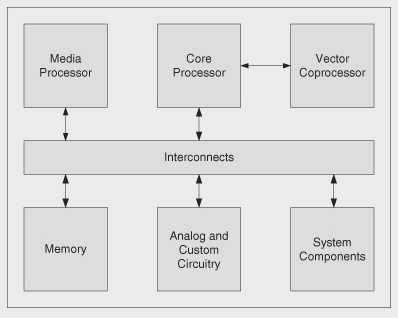
\includegraphics[scale=0.68]{imagens/basicsoc.png}\\
		{\small \textbf{Fonte:} \citeonline{MichelSoC}}
    \end{center}\label{fig:socbasic}
\end{figure}

% Descrição Cyclone V pincipais característica, famílias, imagem 
%================================

Dentre os dispositivos classificados como SoC, a Intel fornece uma linha de produtos classificados como SoC-FPGA, os quais se caracterizam por possuir um rede de FPGA integrados a um processador ARM\@. Uma família de produtos que possuem essa característica é a Cyclone V SoC-FPGA\@. Estes componentes são constituídos por um \textit{Hardware Processor System} (HPS) que possui processadores ARM Cortex-A9 de um ou dois núcleos e um FPGA\@. A Figura~\ref{fig:socfpga} oferece uma visão global da integração entre os dois componentes principais do SoC-FPGA da família Cyclone V. 

\begin{figure}[ht]
	\caption{Diagrama de blocos simplificado Cyclone V}
	\begin{center}
		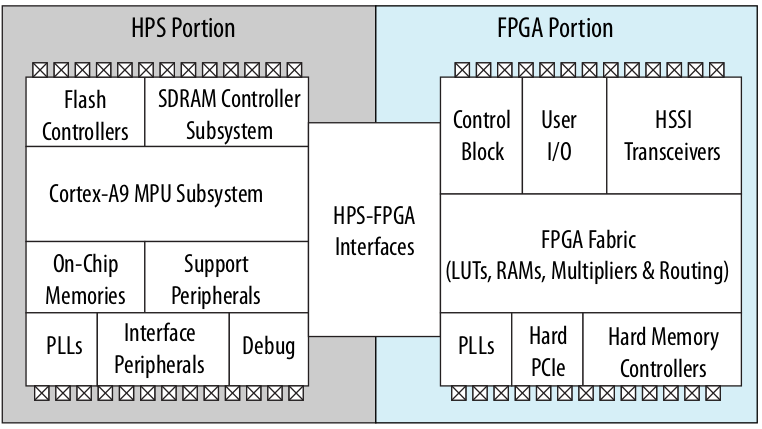
\includegraphics[scale=0.46]{imagens/socfpga.png}\\
		{\small \textbf{Fonte:} \citeonline{alteraCV}}
    \end{center}\label{fig:socfpga}
\end{figure}

Lançada iniciante pela Altera que foi adquirida em 2015 pela Intel~\cite{intelbuyaltera}, a família Cyclone V SoC-FPGA alia o poder de processamento do processador Cortex-A9 à versatilidade e flexibilidade do FPGA, o que faz desta linha de componentes possuir um alto poder de processamento aliado a um baixo consumo. Os caminhos de interconexão entre o HPS e o FPGA do Cyclone V proporcionam altas taxas de transferência, o que seria inviável em sistemas com dois chips. Esta estratégia de integração em um único circuito integrado oferece~\cite{CycloneV}:

\begin{itemize}
    \item Largura de banda de pico de mais de 100 Gbps;
    \item Coerência de dados integrada;
    \item Significativa economia de energia do sistema, eliminando caminhos de E/S externos entre o processador e o FPGA\@.
\end{itemize}

Este nível de integração entre os dois componentes que formam o SoC FPGA provê uma solução com baixa potência dissipada, aliado a um reduzido custo e  espaço da placa necessária para a montagem do sistema. Ou seja, o uso dos SoC-FPGA, com processador ARM combinado com FPGA, interligados através de um \textit{backbone} de alta largura de banda e baixa potência, disponíveis nos produtos da linha da família Cyclone V da Intel, possibilita o desenvolvimento de aplicações com excelente desempenho, alta flexibilidade, além de baixo custo e baixo consumo de energia. 

\section{ARM Cortex-A9}
O processador Cortex A9 é uma linha de processadores ARM otimizados para alcançarem maior desempenho aliado a um baixo consumo. Esta linha de processadores ARM é uma das mais utilizadas, nas mais diversas aplicações. O Cortex A9 possui uma estrutura interna configurável, o que oferece flexibilidade ideal para o desenvolvimento de um novo SoC.  Na Tabela~\ref{tab:cortexA9config} são listadas algumas das configurações básicas do processador Cortex A9.

\begin{table}[ht]
    \caption{Configurações básicas do ARM Cortex A9 }
    \begin{center}    
        \begin{tabular}{ll}
        \hline \hline
        Arquitetura                     & Armv7-A                                     \\ \hline \hline
        Multicore                       & 1-4 cores                                   \\ \hline \hline
        \multirow{7}{*}{Suporte ISA}    & Armv7-A                                     \\ \cline{2-2} 
                                        & Thumb-2 ou Thumb                            \\ \cline{2-2}
                                        & Tecnologia de segurança TrustZone           \\ \cline{2-2}
                                        & Jazelle DBX e Tecnologia RCT                \\ \cline{2-2}
                                        & Extensão DSP                                \\ \cline{2-2}
                                        & Neon (Opcional)                             \\ \cline{2-2}
                                        & Ponto Flutuante (Opcional)                  \\ \hline \hline
        Unidade de Gerenciamento de Memória (MMU)    & Armv7 MMU                      \\ \hline \hline
        Depuração                  & CoreSight                                        \\ \hline \hline
        \multirow{4}{*}{Caracteristicas}& Dual-issue, partially out-of-order pipeline \\ \cline{2-2}
                                        & \begin{tabular}[c]{@{}l@{}}Arquitetura do sistema flexível com
                                            \\caches configuráveis\end{tabular}       \\ \cline{2-2}
                                        & Sistema de coerência com ACP port           \\ \cline{2-2}
                                        & \begin{tabular}[c]{@{}l@{}}Desempenho 50\% maior do que  
                                            \\ o processador Cortex-A8  configurado 
                                            \\ como \textit{single-core}\end{tabular} \\ \hline\hline
        \end{tabular}
        \\{\small \textbf{Fonte:} \citeonline{armCortexA9}}
    \end{center}\label{tab:cortexA9config}
\end{table}

\subsection{Cortex-A9 MPCore Processor}
O Cortex-A9 MPCore processor é formado por três partes. Estas partes são componentes configuráveis que proporcionam a flexibilidade necessária para implementação de sistemas dedicados sob medida para determinada aplicação. Os componentes do Cortex-A9 MPCore são~\cite{mpcore}:

\begin{itemize}
    \item De um a quatro processadores Cortex-A9, que podem ser agrupados em um cluster, e um \textit{Snoop Control Unit} (SCU) que pode ser usado para assegurar a coerência do cluster;

    \item Um conjunto de periféricos de memória mapeada, incluindo timer global, watchdog e timer privativo para cada processador contido no cluster; e
    
    \item Um controlador de interrupção integrado que é uma implementação do Generic Interrupt Controller. 
\end{itemize}

A Figura~\ref{fig:mpcore} apresenta um diagrama que representa o Cortex-A9 MPCore processor.

\begin{figure}[ht]
	\caption{Cortex-A9 MPCore Processor}
	\begin{center}
		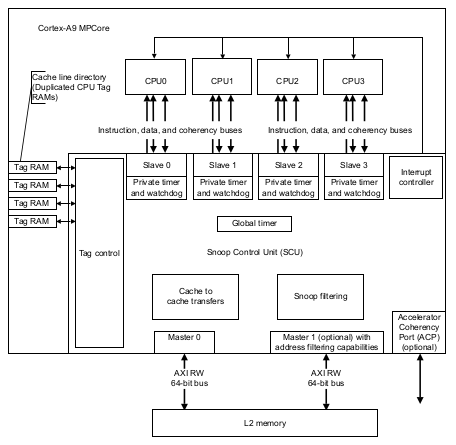
\includegraphics[scale=0.7]{imagens/mpcoreA9.png}\\
		{\small \textbf{Fonte:} \citeonline{mpcore}}
    \end{center}\label{fig:mpcore}
\end{figure}

% \subsection{Protocolo AMBA 3}
% \subsection{Generic Interrupt Control - GIC}

\section{Field-Programmable Gate Array - FPGA}
\textit{Field-Programmable Gate Arrays}, ou simplesmente FPGA, são dispositivos semicondutores construídos através de uma matriz de blocos lógicos configuráveis, os CLBs~\cite{FPGAXilinx}. Estes blocos lógicos são interconectados a partir de conexões programáveis, o que permite ao projetista conectar esses blocos em configurações capazes de executar qualquer tarefa, desde simples portas lógicas até complexas funções.

Os FPGAs foram batizados como dispositivos programáveis em campo devido a capacidade de terem seu hardware reconfigurado pelo usuário, para executar uma função desejada, mesmo após seu processo de fabricação. Esta característica permite que atualizações e soluções de possíveis erros de projetos sejam executadas em campo. São estas características que diferem os FPGAs dos circuitos integrados de aplicação específicas, também conhecidos como ASICs - \textit{Application Specific Integrated Circuits}, que como o nome já sugere, são circuitos desenvolvidos e fabricados para desempenharem apenas uma tarefa específica.

Extremamente versáteis, os FPGAs permitem que desenvolvedores testem inúmeras aplicações mesmo depois que o próprio FPGA e todo o hardware auxiliar já estarem montados em suas placas. Se por algum motivo uma nova configuração for necessária, novos arquivos de configuração podem ser transferidos para o FPGA, fornecendo ao dispositivo novas funcionalidades ou mesmo correção de defeitos. FPGAs são poderosas ferramentas de prototipagem devido à sua flexibilidade, mesmo depois do hardware já estar montado. Aplicações comerciais normalmente usam FPGAs em produtos finais quando a necessidade de computação paralela e requerimentos dinâmicos são um requisito do sistema~\cite{FPGAarm}.



\section{Hardware Processos System}
Como foi mencionado no início deste capítulo, a família de dispositivos Cyclone V system-on-a-chip (SoC) é formada por duas partições, uma malha de FPGA e um processador Arm Cortex-A9, que pode estar organizado em dois ou apenas um núcleo. Esta última partição é chamada de \textit{Hard Processor System} (HPS). 

Os principais módulos do HPS são:

\begin{itemize}
    \item Microprocessador Unit - MPU, subsistema com um ou dois ARM Cortex-A9 (MPCore Processor)
    \item Controladores de memória Flash;
    \item Controladores de SDRAM;
    \item Sistema de interconexão;
    \item On-chip memória; e
    \item Phase-locked loops (PLLs).
\end{itemize}


\subsection{FPGA Manager}
O \textit{FPGA Manager} é o bloco do \textit{Hard Processor System} responsável por gerenciar e monitorar a malha de FPGA presente no SoC. Através do \textit{FPGA Manager} o projetista é capaz de configurar o FPGA, monitora seu estado, além de enviar dados entre o HPS e o FPGA\@. 

\begin{figure}[ht]
	\caption{Diagrama de blocos FPGA Manager }
	\begin{center}
		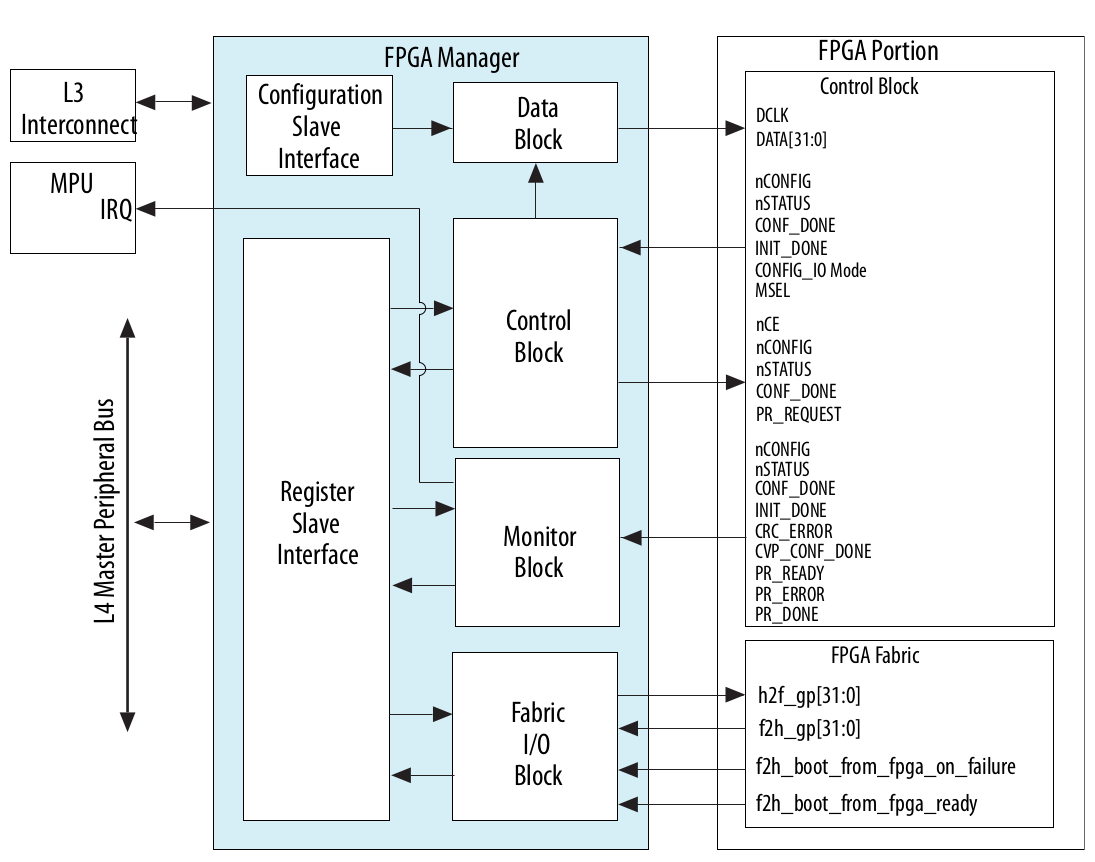
\includegraphics[scale=0.3]{imagens/fpgamanager.png}\\
		{\small \textbf{Fonte:} \citeonline{alteraCV}}
    \end{center}\label{fig:fpgamanager}
\end{figure}

O \textit{FPGA manager} possui as seguintes funcionalidades:

\begin{itemize}
    \item Capacidade de realizar configuração parcial ou completa de toda a malha do FPGA\@;
    \item Enviar 32 sinais de uso geral  do HPS para o FPGA\@;
    \item Receber 32 sinais de uso geral do FPGA para o HPS\@;
    \item Monitorar o status de configuração e potência do FPGA\@;
    \item Gerar interrupções para o HPS a partir das mudanças de status do FPGA\@; e
    \item Capacidade de resetar o FPGA\@.
\end{itemize}

Na Figura~\ref{fig:fpgamanager} podemos ver os principais blocos que formam o sistema do \textit{FPGA Manager}, O \textit{Registrer Slave Interface} se conecta ao L4 \textit{Master Peripheral Bus} fornecendo acesso ao registro de \textit{status} da malha do FPGA\@. Já o \textit{Configuration slave interface} se conecta ao \textit{L3 interconnect} da MPU fornecendo um caminho para que o FPGA possa ser reconfigurado a partir do HPS\@.

Do lado da malha do FPGA, o \textit{FPGA Manager} possui dois blocos, o \textit{fabric I/O} e o \textit{monitor}. No bloco \textit{fabric I/O} os registradores \textit{General-purpose input register} (gpi), \textit{General-purpose output register} (gpo) e \textit{Boot handshaking input register} (misci) possibilitam a comunicação entre o HPS e a malha do FPGA\@. Estes registradores só são acessíveis quando o FPGA está no modo usuário, modo ao qual o FPGA pode ser reconfigurado a partir do HPS\@. O bloco \textit{monitor}, como pode ser deduzido pelo seu nome, fornece uma interface para o monitoramento da malha do FPGA, este bloco monitora sinais relacionados com a configuração do FPGA 


\subsection{HPS-FPGA Bridge}
O HPS pode se comunicar com a malha do FPGA a partir de barramentos de alto desempenho, que podem alcançar larguras de banda superiores a 100Gbps. Estes barramentos, chamados de HPS-FPGA Bridge, usam o protocolo \textit{Advanced Microcontroller Bus Architecture} (AMBA) \textit{Advanced eXtensible Interface} (AXI), o qual foi desenvolvido pela própria ARM, constituindo-se num padrão de conexão dos blocos internos dos dispositivos ARM\@. A Figura~\ref{fig:hpsfpgabridge} exibe o diagrama de blocos das conexões de todas a pontes presentes do Cyclone V.

\begin{figure}[ht]
	\caption{Diagrama de blocos HPS-FPGA Bridge}
	\begin{center}
		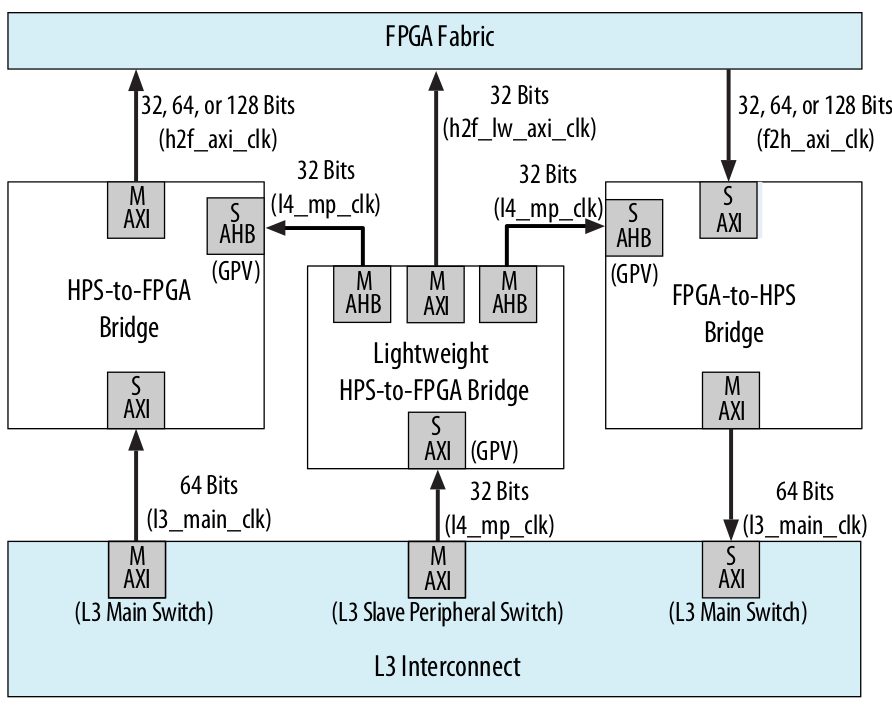
\includegraphics[scale=0.35]{imagens/hps-fpga_bridge.png}\\
		{\small \textbf{Fonte:} \citeonline{alteraCV}}
    \end{center}\label{fig:hpsfpgabridge}
\end{figure}

O HPS possui três pontes, são elas: \textit{FPGA-to-HPS Bridge}, \textit{HPS-to-FPGA Bridge} e a \textit{Lightweight HPS-to-FPGA Bridge}. Estas pontes permitem a comunicação entre o HPS e o FPGA e vice-versa, ou seja, quando o projetista incorpora periféricos ao seu projeto no FPGA, o processador pode acessar esses periféricos através de um barramento de alta velocidade. Como foi dito, essa comunicação também funciona no sentido inverso, do FPGA para o HPS, significando que um componente implementado no FPGA pode acessar regiões de memória e/ou periféricos do HPS\@.


\subsection{Cortex-A9 Microprocessor Unit Subsystem}
Os SoCs da família Cyclone V incluem um \textit{Hard Processor System} formado por um Arm Cortex-A9 MPCore, com processador de uso geral de 32 bits com um ou dois núcleos, um L2 cache, um \textit{Accelerator Coherency Port} (ACP) e módulo de depuração. Tanto o processador como outros módulos no HPS podem acessar blocos lógicos instaciados no FPGA através do \textit{HPS-to-FPGA bridge}. Na Figura~\ref{fig:mpusubsystem} é apresentado um diagrama de blocos simplificado do MPU\@.

\begin{figure}[ht]
	\caption{Cortex-A9 Microprocessor Unit Subsystem com bloco do sistema de interconexão}
	\begin{center}
		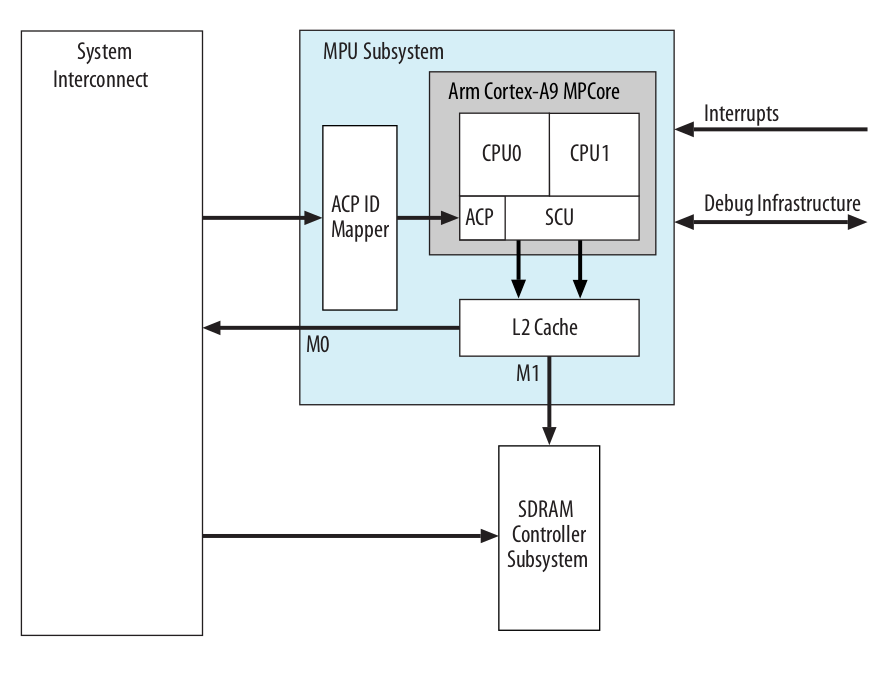
\includegraphics[scale=0.37]{imagens/mpusubsystem.png}\\
		{\small \textbf{Fonte:} \citeonline{alteraCV}}
    \end{center}\label{fig:mpusubsystem}
\end{figure}


\section{Kit de desenvolvimento DE10-nano}

Para o desenvolvimento deste trabalho foi escolhido o kit de desenvolvimento DE10-Nano da Terasic. Construído com base no SoC Cyclone® V SE 5CSEBA6U23I7 integrado com um processador ARM Cortex-A9 dual-core. O kit disponibiliza toda a estrutura básica de hardware necessário para que usuários possam aproveitar todo o poder do hardware reconfigurável oferecido pelo FPGA, combinado com um processador de alto desempenho. Além do SoC Intel, a placa DE10-Nano (Figura~\ref{fig:de10-nano}) oferece excelentes recursos, como memória DDR3 de alta velocidade, conversor analógico-digital, interface USB e interface de rede gigabit ethernet, os quais dão ao kit grande flexibilidade no desenvolvimento de novas aplicações. 

\begin{figure}[ht]
	\caption{Kit de desenvolvimento DE10-Nano}
	\begin{center}
		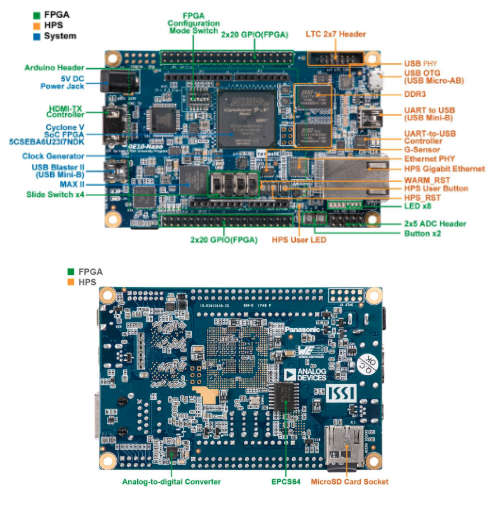
\includegraphics[scale=0.65]{imagens/de10nano.png}\\
		{\small \textbf{Fonte:}\cite{DE10nano}}
    \end{center}\label{fig:de10-nano}
\end{figure}

\chapter{Robot Operating System - ROS}\label{cap:ros}

\begin{citacao}
``O Robot Operating System (ROS) é um conjunto de bibliotecas de software e ferramentas que te auxiliam na construção de aplicações em robótica. De \textit{drivers} ao estado da arte de algoritmos, e com poderosas ferramentas de desenvolvimento, ROS tem o que você precisa para seu próximo projeto de robótica. E tudo é open source~\cite{Ros}''    
\end{citacao}

O ROS foi idealizado com o objetivo de ser um ambiente completo, de código aberto, para elaboração de sistemas robóticos. Largamente aceito e amplamente utilizado atualmente, os desenvolvedores se beneficiam da alta qualidade de código proporcionado pelo grande número de usuários e plataformas que aproveitam-se do ROS em seus projetos~\cite{RosIntro}. Uma ampla variedade de sensores e atuadores empregados na robótica também seguem essa tendência e oferecem suporte ao ROS através de seus~\textit{drivers}. O ROS fornece abstração de hardware, controle de baixo nível para dispositivos, funcionalidades e bibliotecas de uso comum, passagem de mensagens entre processos e gerenciamento de pacotes~\cite{rosEfetiveProgram}. Por esses motivos, o ROS é conhecido como um meta sistema operacional para robôs. Neste capítulo será apresentado o ROS e as vantagens do seu uso na concepção de novas plataformas robóticas.

A cada ano o ROS vem se consolidando como o~\textit{framework} padrão para o desenvolvimento de novos projetos de robótica. Apesar de já possuir esta posição, o ROS possui uma história relativamente curta. O ROS teve início no Laboratório de Inteligência Artificial de Standord e em 2007 a companhia Willow Garage assumiu o seu desenvolvimento. A Willow Garage é uma empresa que desenvolve robôs pessoais e de serviços. Ela também é responsável pelo desenvolvimento de suporte a \textit{Point Cloud Library (PCL)}, que é uma biblioteca de software largamente usada para processamento de nuvens de pontos. Em Janeiro de 2010 a primeira versão do ROS foi lançada, desde então muitas outras versões a sucederam. O ROS está sob as licenças BSD 3-Clause e Apache 2.0, que permite qualquer um modificar, reusar e distribuir códigos ROS~\cite{rosPYO}. Atualmente o ROS se encontra com uma versão estável do ROS2 e o ROS1 tem seu fim marcada para maio de 2025.


\section{Um sistema operacional para robôs}

De forma simplificada um sistema operacional tem como objetivo gerenciar os recursos do sistema computacional, ele atua como uma ponte entre esses recursos e o seu usuário, ou seja, o sistema operacional se faz necessário para disponibilizar às aplicações os recursos funcionais do sistema de forma padronizada, se tornando uma verdadeira camada de abstração entre os programas e o hardware. Windows e Ubuntu, para computadores pessoais, e Android, para smartphones, são exemplos de sistemas operacionais populares.

A comunidade da robótica em todo mundo tem feito grande progresso nos últimos anos. Dispositivos de hardware confiáveis e com menor custo têm sido ofertados em um nível nunca encontrado no passado, desde robôs móveis terrestres, passando por drones e até mesmo robôs humanóides estão disponíveis no mercado com relativa facilidade. O que pode ser até mais impressionante, a comunidade também tem desenvolvido algoritmos que permitem que estes robôs possuam um nível crescente de autonomia. Apesar desse rápido progresso, o desenvolvimento de robôs ainda representam um desafio para os desenvolvedores de software e grande parte desse desafio se deve a falta de padronização de um software específico para robótica, ou até mesmo um sistema operacional dedicado para robôs, como podemos encontrar em outros nichos, como os PCs e smartphones. Neste contexto, o ROS tenta preencher essa lacuna.

O nome ROS vem da abreviação de \textit{Robot Operating System}, mas seria o ROS um sistema operacional para robôs? Ele fornece abstração de hardware, controle de baixo nível para dispositivos, implementações de funcionalidades de uso comum, troca de mensagens entre processos, até um sistema de gerenciamento de pacotes. Além destas características o ROS está equipado com bibliotecas e ferramentas para escrever, compilar e rodar seus códigos~\cite{RosIntro}.

Apesar de todos os atributos que o caracterizam como um sistema operacional, o ROS não é um sistema operacional convencional, por ainda precisar rodar em um outro sistema operacional previamente instalado, o que faz com que o ROS seja conhecido como um meta-sistema operacional. Antes de ter o ROS em execução no robô é necessário instalar um sistema operacional, como por exemplo o Ubuntu. Com a distribuição Linux rodando é possível executar a instalação completa do ROS, sendo assim, todos os recursos fornecidos por um sistema operacional convencional podem ser utilizados pelo ROS, como sistema de gerenciamento de processos, sistema de arquivos, interface do usuário e compiladores, dentre outros. 

Para complementar esses recursos básicos do sistema operacional, o ROS fornece funcionalidades específicas para o uso na robótica, tal como bibliotecas para transmissão e recepção de dados para uma variedade de dispositivos de hardwares comumente utilizados em sistemas robóticos. Esse tipo de software é conhecido como \textit{middleware} ou \textit{framework}. Como pode ser visto na Figura~\ref{fig:rosmeta}, o ROS é o sistema auxiliar para controlar atuadores e sensores, com um nível de abstração de hardware dando suporte para o desenvolvimento de novas aplicações de robótica em sistemas operacionais convencionais.

\begin{figure}[ht]
	\caption{ROS: um meta-sistema operacional}
	\begin{center}
		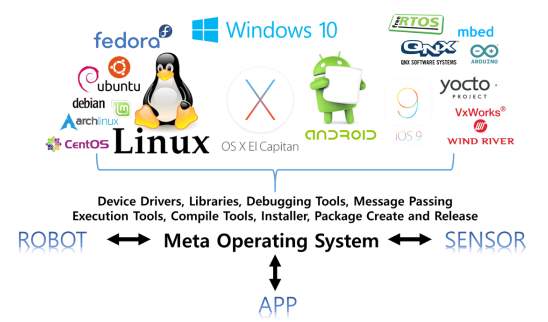
\includegraphics[scale=0.6]{imagens/metaOS.png}\\
		{\small \textbf{Fonte:} \citeonline{rosPYO}}
    \end{center}\label{fig:rosmeta}
\end{figure}


\section{Vantagens do ROS}
Até agora descrevemos o ROS como uma ferramenta ideal para o desenvolvimento de novos projetos de robótica, apesar disto, aprender a usar um novo \textit{framework} é uma atividade árdua, principalmente um tão abrangente e complexo como o ROS\@. Esse tipo de questão deve ser levada em consideração na escolha das ferramentas no inicio de um novo projeto. 

O objetivo do ROS não é ser um \textit{framework} com o maior número de recursos, seu principal objetivo é oferecer o máximo de reuso de software usados no desenvolvimento de novos robôs. O ROS é um \textit{framework} de computação distribuída, isso que dizer que os seus processos podem ser projetados individualmente e podem ser integrados ao sistema livremente e em tempo de execução. Estes processos podem ser agrupados em pacotes, facilitando o compartilhamento e a sua distribuição. Outra iniciativa para incentivar a colaboração e o compartilhamento de código são os repositórios oficiais do ROS, que estão disponíveis de forma livre. 

A seguir serão listadas algumas características que incentivam a colaboração da comunidade e são responsáveis pelo sucesso do ROS\@:

\begin{itemize}
    \item\textbf{Recursos Nativos:} O ROS oferece, de forma nativa, muitos recursos prontos, testados e validados pela comunidade. Podemos citar como exemplos o \textit{Simultaneous Localization and Mapping (SLAM)} e o \textit{Adaptive Monte Carlo Localization (AMCL)} que são usados para navegação autônoma de plataformas robóticas móveis. Outro pacote oferecido pelo ROS é o MoveIt, pacote usado para planejamento de movimento de manipuladores. Estes recursos podem ser usados sem problema algum e são altamente configuráveis, podendo ser adaptados em vários modelos de robôs e atender a inúmeras aplicações. 

    \item\textbf{Ferramentas de desenvolvimento:} O ROS é disponibilizado com uma grande quantidade de ferramentas para debugging, visualização, incluindo ferramentas para simulação. Algumas das ferramentas open source mais poderosas para visualização, debugging e  simulação, respectivamente, rqt\underline{ }gui, RViz e Gazebo, são nativas do ambiente ROS\@.
    
    \item\textbf{Suporte a sensores e atuadores:} Muitos dos sensores e atuadores usados na robótica já são suportados pelo ROS e o número de dispositivos compatíveis aumenta a cada ano. Algumas companhias se beneficiam pelo fato de muitos desses dispositivos fazerem uso de hardware aberto e o software existente também pode ser reutilizado a custo zero, fazendo com que o processo de desenvolvimento de novos hardware periféricos usados na robótica também acelere. Sensores como Velodyne-LIDAR e atuadores como os servos Dynamixel, podem ser integrados ao ROS sem impedimento algum.
    
    \item\textbf{Múltiplas linguagens:} O framework ROS pode ser programado em algumas linguagens de programação modernas. Podemos escrever código eficiente em C ou C++ e outra aplicação ser escrita em python. O ROS possui bibliotecas clientes para C/C++, Python, Java e Lisp. Este tipo de flexibilidade não é comum em outros \textit{frameworks}.
    
\end{itemize}


\subsection{Computacão distribuida}
Grande parte de robôs modernos possuem diferentes unidades de processamento, que podem estar localizadas em diferentes computadores. Desde sensores microprocessados até mesmo controles específicos para motores, tais dispositivos podem possuir suas próprias unidades computacionais. Mesmo possuindo apenas um computador, dividir o processamento em processos individuais específicos para cada função e fazer com que eles trabalhem em conjunto na resolução de um problema maior, é uma excelente abordagem para a arquitetura de robôs modernos. Além disso, múltiplos robôs podem trabalhar de forma colaborativa dividindo atividades entre eles, ou até mesmo interagindo com seres humanos que poderiam enviar comandos através de um computador ou celular. Em todos estes casos, é necessário a comunicação entre processos, que podem ou não estarem no mesmo computador. 

O ROS é um \textit{Inter-process communication framework} e de fato ele usa uma rede TCP/IP para realizar essa comunicação entre processos. Ele usa sockets TCP/IP para transportar dados entre os processos. Esta abordagem proporciona grande flexibilidade na troca de mensagem: processos podem se comunicar com outros mesmo se eles não estiverem na mesma máquina, ou até mesmo em robôs separados, bastando para tal que todas as máquinas que compartilham estejam na mesma rede. Isso faz com que até mesmo processos rodando na internet possam participar da comunicação e realizar uma parte do processamento de um robô.


\subsection{Reuso de Software}
O uso do ROS pode diminuir a necessidade de implementar algoritmos que já foram testados e validados por outros pesquisadores. Algoritmos de navegação, planejamento de rotas e mapeamento, dentre outros, são usados em diferentes projetos, e o ROS permite que estes algoritmos sejam reaproveitados de duas maneiras possíveis:

\begin{itemize}
    \item \textbf{Pacotes padrão:} São pacotes de software de importantes algoritmos usados na robótica ou mesmo drivers de dispositivos comuns na robótica, que já foram implementados e testados.

    \item \textbf{Interface de troca de mensagens:} A interface utilizada pelo ROS vem se tornando um padrão na comunicação entre processos em robôs.
\end{itemize}

Nos repositórios oficiais do ROS estão disponíveis centenas de pacotes públicos que utilizam a interface de troca de mensagens padronizada do ROS possibilitando uma redução significativa do esforço necessário para o desenvolvimento de uma lógica para integrar estes pacotes ao seu sistema. Assin, desenvolvedores que usam o ROS podem concentrar mais tempo e esforços no desenvolvimento de suas novas ideias, aproveitando algoritmos consolidados dos repositórios oficiais do ROS, sem a necessidade de reescrevê-los para adaptá-los ao seu projeto.


% \subsection{Testes Rápidos}


\section{Sistema de aquivos}
Como era de se esperar de um sistema operacional, o ROS também possui um sistema de arquivos padronizado. É de extrema importância para o desenvolvimento de novas aplicações conhecer a organização dessa estrutura de arquivos. A Figura~\ref{fig:rosfile} apresenta um diagrama de blocos do sistema de arquivo do ROS\@.

\begin{figure}[ht]
	\caption{Sistema de arquivos ROS}
	\begin{center}
		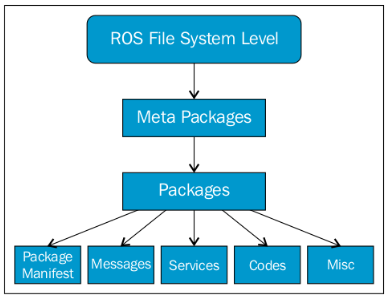
\includegraphics[scale=0.7]{imagens/fileSiystem.png}\\
		{\small \textbf{Fonte:} \citeonline{rosMastering}}
    \end{center}\label{fig:rosfile}
\end{figure}

A seguir são apresentados a definição de cada bloco da estrutura de arquivos do ROS\@:
\begin{itemize}
    \item \textbf{Pacotes:} Pacotes são a unidade de software principal do ROS\@. Um pacote pode conter nós, dependências, bibliotecas, datasets, arquivos de configuração, ou qualquer coisa que seja útil organizar de forma agrupada~\cite{RosPKG}.

    \item \textbf{Manifesto do pacote:} O arquivo package.xml é conhecido como manifesto do pacote, ele fornece os metadados a respeito do pacotes, incluindo nome, versão, descrição, licença, dependências e outras informações. Os padrões do package.xml são definidos no REP-0127.
    
    \item \textbf{Metapackages:} Metapackages são pacotes especializados que serve apenas como representante de um grupo de outros pacotes relacionados entre si.
    
    \item \textbf{Meta packages manifest:} O manifesto de um metapackage é semelhante ao manifesto de um pacote comum, a diferença entre eles é que no manifesto devemos incluir as dependências encontradas no mesmo repositório do meta package
    
    \item \textbf{Message (msg) types:} É o arquivo de descrição de um tipo de mensagem, é armazenado no diretório my\underline{ }package/msg/MyMessageType.msg e define toda a estrutura de dados enviados a partir deste tipo de mensagem.
    
    \item \textbf{Service (srv) types:} É o arquivo de descrição de um tipo de mensagem, é armazenado no diretório my\underline{ }package/srv/MyServiceType.msg e define toda a estrutura de dados enviados a partir deste tipo de serviço.
    
    \item \textbf{Repositórios:} Pacotes ROS são compartilhados usando algum tipo de Version Control System (VCS), como o gti. Cada repositório pode conter apenas um pacote ou um metapackage 
\end{itemize}


\subsection{Pacotes ROS}

A unidade básica para configuração do software no ROS é conhecida como pacote, isso quer dizer que todas as aplicações desenvolvidas para ROS são estruturadas como um pacote. Na Figura XX podemos ter uma visão da estrutura típica de uma pacote ROS

\begin{figure}[ht]
	\caption{Estrutura típica de um pacote ROS ROS}
	\begin{center}
		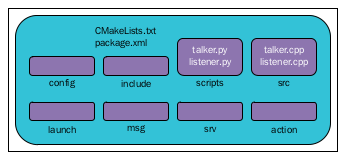
\includegraphics[scale=0.8]{imagens/rospackagestruture.png}\\
		{\small \textbf{Fonte:} \citeonline{rosMastering}}
    \end{center}\label{fig:rospacotestrut}
\end{figure}

Nos pacotes estão contidos um ou mais nós, como são chamadas as unidades de processamento no ROS, ou podem incluir arquivos de configuração para a execução de nós de outros pacotes. Existem milhares de pacotes ROS oficiais e uma quantidade ainda maior de pacotes desenvolvidos por seus usuários. 

Cada metapackage possui um arquivo chamado package.xml, este arquivo é responsável por reunir informações importantes sobre o pacote, nele podemos encontrar o nome do pacote, seu autor, dependências e licença de uso. O sistema de compilação do ROS é o Catkin, ele usa o CMake e o arquivo CMakeLists.txt que deve estar dentro da pasta de cada pacote com as suas instruções de compilação. 

Os pacotes são as menores unidades que podem ser compiladas no ROS, são também  a maneira com que podemos organizar o software para ser lançado. No caso dos pacotes oficiais do ROS, por exemplo, existe um pacote Debian, que são os pacotes utilizados pelo Ubuntu, para cada pacote ROS. Apesar do conceito ser semelhante, e mesmo que ao instalar um pacote Debian, você possa incluí-lo à sua lista de pacotes ao ROS instalado no sistema, os pacotes debian e ROS não são equivalentes. 

A principal função dos pacotes é ser uma maneira funcional, de fácil configuração e um caminho descomplicado para possibilitar o reuso de software. De maneira geral o pacotes ROS devem conter funcionalidades suficientes para serem úteis, mas não muito para torná-los muito grande e confuso, tornando seu uso difícil por outro software 


\subsection{Mensagens ROS}
Os nós do ROS podem publicar apenas dados de tipos predeterminados. Estes tipos são definidos usando uma linguagem de descrição de mensagens, conhecida como ROS messages. Esta simples descrição permite que as ferramentas do ROS gerem automaticamente o código fonte para mensagens para todas as linguagens aceitas no ROS\@. As descrições das mensagens são armazenadas no arquivo .msg localizada no subdiretório msg/ dentro de um pacote ROS\@.

Existem dois segmentos em um arquivo .msg, são eles: Fields e constants. Filds são os dados que serão enviados dentro da mensagens. Constants define os valores, ou tipo de dados, que poderão ser usados em cada campo. Os tipos de mensagens são referenciados a partir do nome do seu respectivo pacote, como ilustração, podemos usar o arquivo de descrição geometry\underline{ }msgs/msg/Twist.msg, que será referencido como geometry\underline{ }msgs/Twist. 

O ROS possui um grande número de mensagens predefinidas, o que não impede que o programador escreva seus próprios arquivos .msg com a descrição de uma mensagem específica para atender a sua aplicação. A Tabela~\ref{tab:rostype} a seguir lista os tipos de dados padrão do ROS que podem ser usados na criação de novas mensagens: 

\begin{table}[ht]
	\caption{Estrutura típica de um pacote ROS }
    \begin{center}
        \begin{tabular}{llll}
        \hline
        \textbf{Primitive type} & \textbf{Serialization} & \textbf{C++} & \textbf{Python} \\ \hline\hline
        bool(1)     & unsigned8-bitint              & uint8\_t(2)  & bool            \\ 
        int8        & signed8-bitint                & int8\_t      & int             \\ 
        uint8       & unsigned8-bitint              & uint8\_t     & int             \\ 
        int16       & signed16-bitint               & int16\_t     & int             \\ 
        uint16      & unsigned16-bitint             & uint16\_t    & int             \\ 
        int32       & signed32-bitint               & int32\_t     & int             \\ 
        uint32      & unsigned32-bitint             & uint32\_t    & int             \\ 
        int64       & signed64-bitint               & int64\_t     & long            \\ 
        uint64      & unsigned64-bitint             & uint64\_t    & long            \\ 
        float32     & 32-bitIEEEfloat               & float        & float           \\ 
        float64     & 64-bitIEEEfloat               & double       & float           \\ 
        string      & asciistring(4)                & std::string  & string          \\ 
        time        & Secs/nsecs signed 32bit ints  & ros::Time    & rospy.Time      \\ 
        duration    &S ecs/nsecs signed 32bit ints  & ros::Duration& rospy.Duration  \\ \hline
        \end{tabular}
        \\{\small \textbf{Fonte:} \citeonline{rosLearning}}
    \end{center}\label{tab:rostype}

\end{table}


\subsection{Workspace ROS}
De forma geral, o workspace é uma pasta no computador que contém todos os pacotes que estão sendo usados no desenvolvimento de uma nova aplicação. Estes pacotes contêm os arquivos fontes e o workspace fornece um local para que os pacotes sejam compilados. O workspace se torna ainda mais útil quando é necessário compilar vários pacotes ao mesmo tempo, todos os pacotes poderão estar contidos no mesmo workspace centralizando todo processo de desenvolvimento. Não existe um diretor específico para que o workspace seja criado, logo, ele pode ser criado no local de preferência do desenvolvedor e sua equipe. Um workspace típico é mostrado na Figura~\ref{fig:rosworkspace}. 

\begin{figure}[ht]
	\caption{Estrutura típica de workspace ROS}
	\begin{center}
		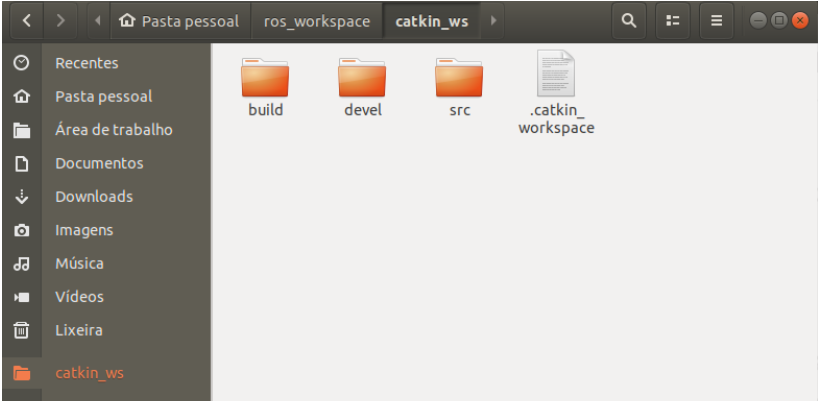
\includegraphics[scale=0.43]{imagens/rosworkspace.png}\\
		{\small \textbf{Fonte:} do Autor}
    \end{center}\label{fig:rosworkspace}
\end{figure}

Cada pasta dentro do workspace é um diferente espaço diferente, cada um com uma função específica:

\begin{itemize}
    \item \textbf{O espaço das fontes:} No espaço das fontes, localizada na pasta src do workspace, estão localizados todos os pacotes do projetos. O arquivo mais importante dessa área do workspace é o CMakeLists.txt. Este arquivo é gerado na primeira vez em que o workspace é compilado

    \item \textbf{O espaço de compilação:} Localizado na pasta build,é neste local que são armazenadas as informações de cache, configurações e outros arquivos intermediário para que os pacotes sejam compilados corretamente.

    \item \textbf{O espaço de desenvolvimento:} Na pasta de que se encontra o espaço de desenvolvimento, aqui são armazenados os programas compilados. Assim você pode testar seus programas sem a necessidade de instalá-los no sistema.
\end{itemize}

Outra função importante do ROS que pode ser usada através de um workspace é o overlays. Se você tiver um pacote instalado em seu sistema, mas quiser testar uma versão mais atual do mesmo pacote, não é necessário instalar a versão mais atual, você pode baixar o código fonte do pacote dentro do seu workspace, após compilar o workspace o ROS entende que deverá usar a versão presente no workspace e não a versão instalada no sistema.


\section{Compunentes ROS}

\subsection{ROS node}
No ROS os executáveis são chamados de nós, eles podem se comunicar com outros processos por meio dos tópicos, serviços ou pelo servidor de parâmetros. Os nós proporcionam grande modularidade aos sistemas robóticos que usam o ROS, isso faz com que o desenvolvimento destes sistemas se tornem bem mais simples.

Ao ser executado o nó possui um nome único no sistema. Através desse nome o nó pode se comunicar com outros nós. O ROS permite que os nós sejam escritos em diferentes linguagens de programação, as bibliotecas que fornecem a interface do ROS com uma linguagem específica é chamada de biblioteca cliente, as mais populares são: roscpp, para a linguagem C++ e a rospy para a linguagem Python.

Uma característica bastante interessante dos nós ROS é a possibilidade de parâmetros serem modificados no momento em que o nó é iniciado. Esta característica proporciona maior flexibilidade aos nós, já que o uso de parâmetros oferece a possibilidade de o código ser reconfigurado sem a necessidade de recompilar o código fonte, sendo assim podemos adaptar o nó a diferentes cenários sem conhecer detalhes de sua implementação. 


A powerful feature of ROS nodes is the possibility of changing parameters while you start the node. This feature gives us the power to change the node name, topic names, and parameter names. We use this to reconfigure the node without recompiling the code so that we can use the node in different scenes.


\subsection{ROS Topic}

Os tópicos são a maneira com que os nós enviam dados no ROS\@. Mesmo sem uma conexão direta entre dois nós, os tópicos podem ser transmitidos, isso faz com que a geração e o consumo de dados sejam desacoplados. Um tópico pode ser lido por vários nós e de maneira igual, também pode ser publicado por vários nós, mas não é uma boa prática um mesmo tópico ser publicado por nós distintos, isso pode causar conflitos nas informações enviadas. A Figura~\ref{fig:rostopic} ilustra o processo de comunicação com tópico.

\begin{figure}[ht]
	\caption{Comunicação a partir de tópicos ROS}
	\begin{center}
		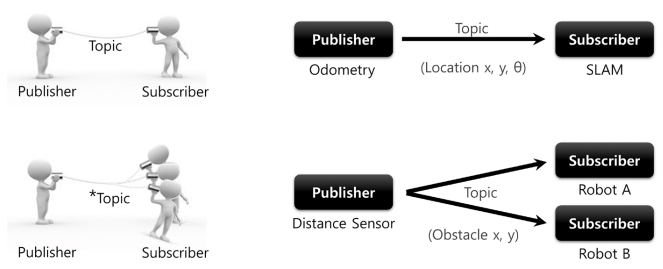
\includegraphics[scale=0.51]{imagens/rostopic.png}\\
		{\small \textbf{Fonte:} \citeonline{rosPYO}}
    \end{center}\label{fig:rostopic}
\end{figure}

As mensagens ROS determinam os tipos de dados que poderão ser transportados através dos tópicos, isso faz com que os tópicos sejam fortemente tipados, consequentemente os mesmo tipo de mensagem deve ser obrigatoriamente o mesmo, para o nó que publica e para o nó que ler um determinado tópico. Sendo assim uma comunicação entre nós, por meio de tópicos apenas ocorrerá se ambos, nó de leitura e nó de publicação, estiverem registrados no ROS master com tópicos de mesmo nome e usando a mesma mensagem.


\subsection{ROS master}

O ROS master é o responsável por registrar nomes dos elementos que fazem parte do sistema, entre eles estão os nós, tópicos, serviços, action, tipos de mensagens, URI w as portas para conexões diretas entre nós, ele também é o encarregado por fornecer o servidor de parâmetros. Por gerenciar as informações das conexões entre as trocas de mensagens entre os nós, o mater ŕ o primeiro elemento que deve ser executado no ROS. Afunção do master é permitir que um determinado nó encontre outro, uma vez localizados os nós poderão se comunicar através de uma conexão per-to-per.

No momento em que um nós é executado no sistema, ele registra seu nome no master. Sendo assim, o ROS master possui os detalhes de todos os nós rodando no sistema. No momento em que qualquer detalhes de um nós muda, ele gera um callback para atualizar as novas informações no master. Quando um nó inicia a publicação de um tópico ele informará todos os detalhes ao master, desde do nome até o tipo de dados que serão enviado, em seguida, o master verifica se existe algum outro nó lendo o mesmo tópico, se algum nó estão querendo fazer a leitura deste tópico o ROS master irá compartilhar detalhes do nó que está publicando com o nós que quer ler o tópico.

Na Figura~/ref{fig:rosMastering} podemos ver como se da a interação entre o master e os nós que farão a comunicação.


\begin{figure}[ht]
	\caption{Gerenciamento de comunicação através do ROS master}
	\begin{center}
		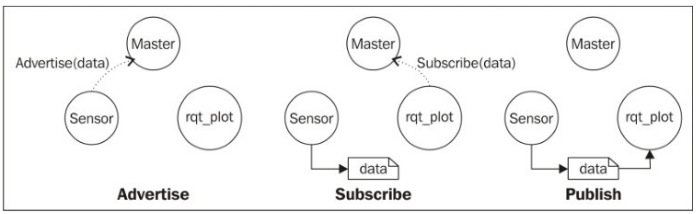
\includegraphics[scale=0.51]{imagens/rosmaster.png}\\
		{\small \textbf{Fonte:} \citeonline{rosEfetiveProgram}}
    \end{center}\label{fig:rosMastering}
\end{figure}

\subsection{ROS Parameters}

Parameters are global variables used in nodes and in the larger context, they can also be considered as a message communication. Parâmetros são variáveis globais que podem ser usadas por nós. Os parâmetros são criados com valores padrões, que podem ser lidos ou escritos por algum processo dentro do sistema ROS. 

O principal objetivo dos parâmetros é fornecer ao sistema a capacidade de se adaptar a cenários distintos de maneira ágil. Por exemplo, o desenvolvedor pode criar um nó para leitura de uma câmera USB, dando à esse nós parâmetros para que usuários desse nós possam configurar o frame rate em que os dados serão publicados, o nome da porta USB em que a câmera está conectada, entre outros, sempre ficando a critério do desenvolvedor. Em casos especiais os parâmetros poderão ser atualizados em tempo de execução, uma função muito útil principalmente em sistemas dinâmicos, que opera em constante mudança.







% No ROS um processo é conhecido como nó, que pode receber e enviar mensagens para se comunicar com outros nós através de uma rede rodando o protocolo TCPROS [3].a busca por sistemas com um grau maior de autonomiaA robótica tem se caracterizádo pelo grande nível de percepção do ambiente e pelos sistemacomplexos de controle do movimentos 

% Com essa distribuição de tarefas através de vários nós podemos criar sistemas cada vez mais complexos, apenas inserindo novos nós na rede, essa rede é gerenciada pelo ROS Master, que é apensas mais um nó do sistema, mas com a função de ser um servidor de nome e serviços para o restante dos nós. Ele identifica os nós na rede, assim todos os nós podem se comunicar com os outros através de conexões peer-to-peer, igura 1. Para desenvolver novas aplicações para o crescente grupo de pacotes ROS, o desenvolvedor deve respeitar os protocolos de comunicação da rede, as bibliotecas do ROS facilitam este trabalho, por já fornecer funções prontas para o desenvolvimento de novos códigos compatíveis e que possam se registrar na rede. Detalhes dos  rotocolos e interno podem ser visto em (ROS, 2011a), (ROS, 2018) e (ROS, 2011b).



% Desenvolver um robô não é algo trivial, atividades que seriam facilmente executadas por nós, seres humnos, como por exemplo, andar de um ponto ao outro de uma sala, do ponto de vista de um robô pode ser um trabalho extremamente árduo. Montar o sistema que possibilite o robô executar as funções pra o qual foi projetado pode facilmente necessitar de um arranjo complexo entre componetes de software e hardware e que pode variar bastante dependendo do ambiente ao qual o robô será exposto. Sendo assim, o desenvolvimento de um sistema robôtico completo necessita de uma conhecimento abrangente e de áreas distintas.  

% Nesse paronama que o ROS foi concebido, com o objetivo de  ser um um ambiente completo para desenvolvimento de sistemas robôticos, facilitando o desenvolvimento com o máximo de reuso de código possibilitando o mínimo de mudanças na adaptação um sistema a um novo ambiente ou até mesmo no desenvolvimento de uma nova plataforma. Atualmente o ROS é um framework bem aceito e amplamente utilizado não apenas na comunidade acadêmica mas também na industria. Desenvolvido originalmente em 2007 no \textit{Stanford Artificial Intelligence Laboratory - SAIL}, a partir de 2008 o ROS foi continuado pela Willow Garage, entretanto em 2012 com a criação da \textit{Open Source Robotics Foundation, Inc. - OSRF} os ROS e projetos parceiros como o Gazebo passaram a ser mantidos pela própria OSRF, que continua o desenvolvimento adicionando novas fancionalidades ao projeto. Além disso muitas instituições de pesquisa adaptaram seus projeto ao ROS, aumentando a cada ano o número de pesquisadores e desenvolvedores trabalhando no aperfeiçoamento do ROS. No site oficial do ROS podemos ver uma lista com diverssas plataformas que utilizam o ROS em seus projetos. http://wiki.ros.org/Robots





% It uses graph architecture with a centralized topology, where processing takes place in nodes that may receive and send messages to communicate with other nodes on the graph net. A node is any process that can read data from a sensor, control an actuator, or run high level, complex robotic or vision algorithms for mapping or navigating autonomously in the
% environment.\cite{rosEfetiveProgram}




% Distributed process: It is programmed in the form of the minimum units of executable processes (nodes), and each process runs independently and exchanges data systematically. Package management: Multiple processes having the same purpose are managed as a package so that it is easy to use and develop, as well as convenient to share, modify, and redistribute. Public repository: Each package is made public to the developer’s preferred public repository (e.g., GitHub) and specifies their license. API: When developing a program that uses ROS, ROS is designed to simply call an API and insert it easily into the code being used. In the source code introduced in each chapter, you will see that ROS programming is not much different from C++ and Python. These characteristics of ROS have allowed users to establish an environment where it is possible to collaborate on robotics software development on a global level. Reusing a code in robot 





\part{Desenvolvimento}
\chapter{Arquitetura do sistema}\label{cap:arquitetura}

Para conseguirmos estabelecer a comunicação entre o computador e o SoC é necessário:

\begin{enumerate}
	\item Efetuar programação de \textit{sockets} e bibliotecas específicas para trabalho em redes; 
	
	\item Desenvolver um pacote ROS para disponibilizar os dados recebidos dos outros pacotes ROS do sistema para o SoC, por meio da interface de rede. 
	
	\item Estabelecer a comunicação entre a interface de rede da placa DE10-nano através de um programa executado no HPS do SoC, que realizará a captura dos dados recebidos através da rede, enviando-os à aplicação sendo executada no FPGA e devolvendo-os ao ROS através da rede. 
\end{enumerate}

Em relação à aplicação embarcada no FPGA contido no SoC, deverá ser descrita por alguma linguagem de descrição de hardware, como por exemplo, Verilog ou VHDL\@.

Todas essas etapas descritas anteriormente são necessárias para a construção completa do sistema proposto, o que torna o desenvolvimento da solução completa um desafio devido às diferentes ferramentas de software e hardware necessárias para sua conclusão. Tendo em vista este problema, a solução foi idealizada para conter o maior grau de modularidade possível, ou seja, cada uma dessas etapas será tratada com um projeto independente, apenas tendo cuidado para garantir a correta comunicação entre cada uma delas.

A grande vantagem que esse abordagem traz ao projeto é a possibilidade futura, tanto da continuação do desenvolvimento como da manutenção do sistema, serem realizados por profissionais com \textit{background} nas diferentes áreas envolvidas, sem a necessidade de se envolver no desenvolvimento de outros módulos. Sendo assim, um profissional especialista em descrição de hardware poderia se dedicar apenas à concepção da solução embarcada no FPGA, sem a necessidade de possuir conhecimento em programação de redes. 

\section{Modelo cliente-servidor}
A comunicação entre o \textit{host}, rodando o ROS, e a placa DE10-nano será estabelecida através de uma rede gigabit ethernet ponto a ponto, ou seja, o host e o SoC estarão conectados diretamente entre si. Desta maneira é possível obter o melhor desempenho da rede, alcançando as maiores taxas de transmissão de dados. Com o meio de comunicação definido, é preciso definir também a arquitetura da comunicação: uma boa alternativa é o modelo cliente-servidor.

O modelo cliente-servidor é caracterizado por possuir uma estrutura que permite dividir o trabalho computacional entre os participantes da comunicação, isto é, entre o servidor, que é o encarregado de disponibilizar os recursos e serviços, e o cliente, que realiza as solicitações para os serviços disponíveis.  Desta maneira tanto o cliente quanto o servidor foram tratados como módulos independentes durante o desenvolvimento do trabalho. O uso do modelo cliente-servidor contribui de forma significativa para que o sistema alcance o máximo de modularização, o que facilita, entre outras coisas, a depuração e manutenção do código, proporcionando mais agilidade e simplicidade no processo de desenvolvimento da solução.


Na Figura~\ref{fig:arquitetura} podemos ter uma visão global do sistema, com destaque a cada etapa da comunicação. No lado do \textit{host}, está instalado o ROS, nele também é onde o cliente será executado, assim sendo o cliente fica responsável por ler o tópico de entrada, fornecido por outro nó do sistema, realizar uma solicitação ao servidor enviando os dados já lidos. O servidor, por sua vez, aceita a solicitação do cliente, recebe os dados e os envia à aplicação embarcada no FPGA que os devolve após seu processamento. Para completar o ciclo, o servidor retorna os dados processados ao cliente, que por sua vez, disponibiliza os dados já processados através do tópico de saída. 

\begin{figure}[ht]
	\caption{Arquitetura geral}
	\begin{center}
		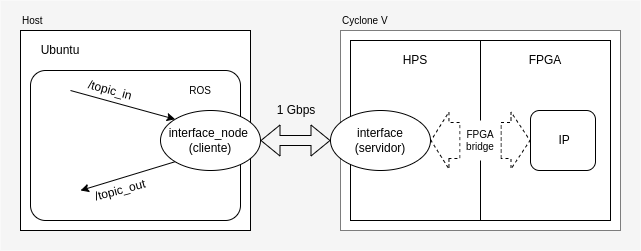
\includegraphics[scale=0.7]{imagens/arquitetura_geral.png}\\
		{\small \textbf{Fonte:} do autor}
    \end{center}\label{fig:arquitetura}
\end{figure}




\section{Biblioteca de comunicação - libinterfacesocket}

Para manter o padrão do desenvolvimentos dos códigos tanto do cliente quanto do servidor, foi desenvolvida uma classe que fornece os métodos para a abertura da comunicação, além de métodos para envio e recebimento das mensagens através da rede gigabit ethernet. Essa classe foi desenvolvida como um módulo à parte e compilada como uma biblioteca estática. Desta forma, uma vez testados e validados seus  métodos de comunicação, tanto o código do cliente quanto o do servidor poderão fazer uso desta biblioteca, eliminando assim a necessidade de reescrever uma parte do código. Outra vantagem nessa abordagem é que, ao manter o código desassociado tanto do servidor como do cliente, nos possibilita fazer alterações ou correções de erros, sem necessariamente realizar alterações nos códigos do servidor ou do cliente.

A programação da biblioteca foi realizada com base em \textit{sockets}. \textit{Sockets} são um caminho para conectar processos em uma rede de computadores. A conexão através de \textit{sockets} entre nós em uma rede independe do protocolo. Um nó da rede ouve uma determinada porta para um IP específico esperando por um pedido de conexão do segundo nó, assim a conexão entre dois processos é estabelecida. O servidor é o nó que aguarda o pedido ser enviado pelo cliente.

A programação de sockets em C++ possibilita um alto nível de otimização da comunicação entre os processos, principalmente por se tratar de um modelo cliente-servidor onde só existirá a comunicação entre o servidor e apenas um cliente. Após implementar a comunicação entre o servidor e o cliente, poderão ser testadas novas técnicas para otimizar o desempenho da rede possibilitando o aumento da taxa de transferência de dados entre o servidor e o cliente.

O código fonte da biblioteca pode ser encontrado no repositório no github~\cite{Pereira-Neto-Biblioteca}, que pode ser visto na figura~\ref{fig:gitlib}, onde podemos observar a estrutura de arquivos da blibioteca. Vale frizar que, a libinterfacesocket possui um makefile para realizar o processo de compilação de forma automática. Assim podemos de forma simplificada compilar e instalar a biblioteca tanto no sistema do host onde será executado o cliente, quanto no sistema do HPS embarcado no SoC, onde o servidor estará rodando. 

\begin{figure}[ht]
	\caption{Repositório libinterfacesocket}
	\begin{center}
		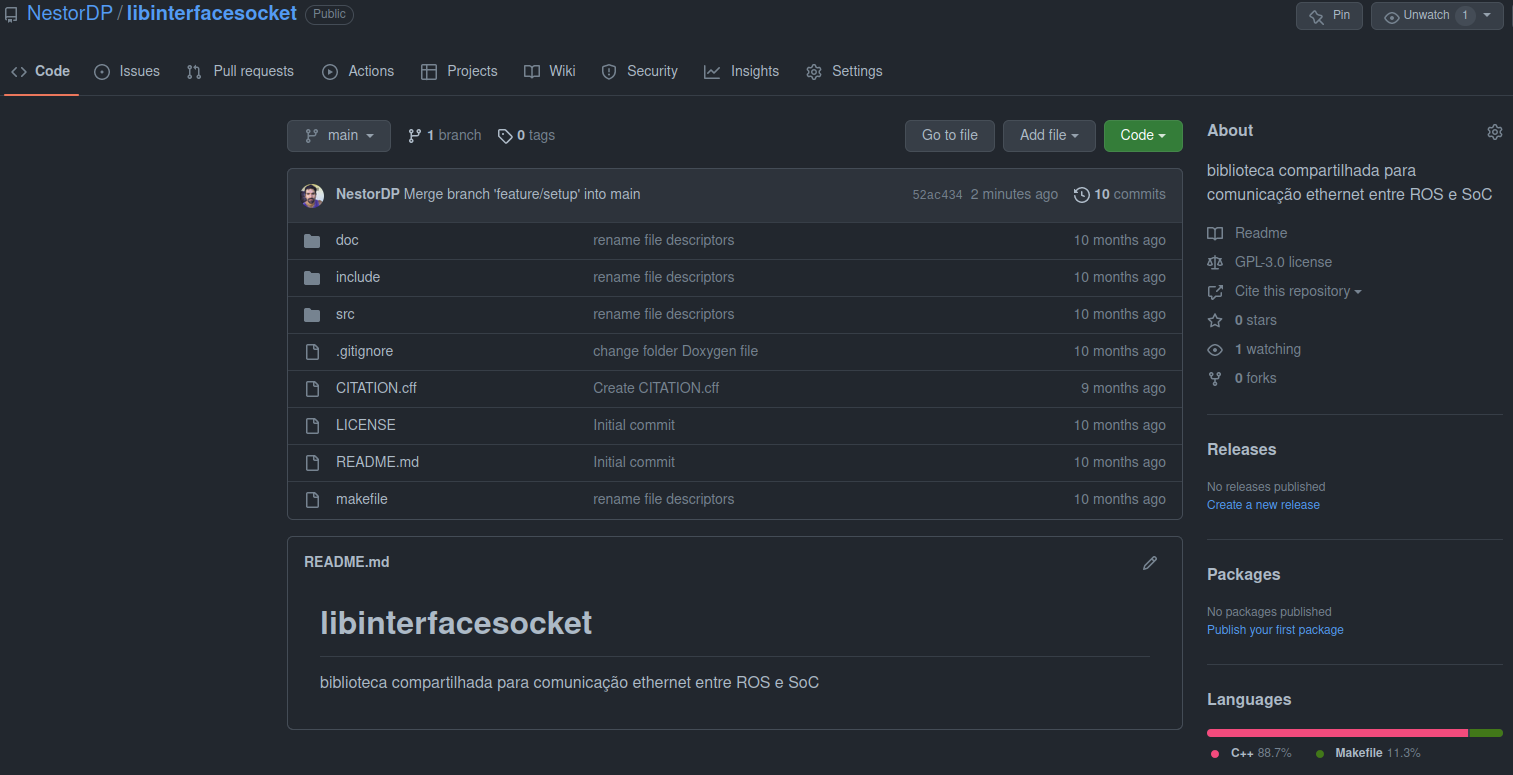
\includegraphics[scale=0.26]{imagens/git_libinterfacesocket.png}\\
		{\small \textbf{Fonte:} do autor}
    \end{center}\label{fig:gitlib}
\end{figure}

\chapter{Pacote ROS (cliente)}\label{cap:cliente}

Como já foi mencionado anteriormente, o cliente é um pacote ROS, sendo assim, deve-se levar em consideração os conceitos de programação do framework ROS em seu desenvolvimento. As técnicas específicas de programação ROS usadas no cliente serão descritas com detalhes neste capítulo, além da explicação do seu funcionamento interno e do uso da libinterfacesocket.

No desenvolvimento de aplicações com ROS deve ser respeitada a estrutura de diretórios  de um pacote ROS\@. Pacotes são a maneira com que os softwares são organizados no ROS, eles podem conter desde nós, que são a unidades de processamento do ROS, até mesmo bibliotecas ou módulos de softwares de terceiros. Os pacotes devem seguir uma estrutura padrão, por este motivo o código fonte do cliente foi organizado como é mostrado na Imagem~\ref{fig:clientdiretorios}.

\begin{figure}[ht]
	\caption{Estrutura de diretórios pacote cliente}
	\begin{center}
		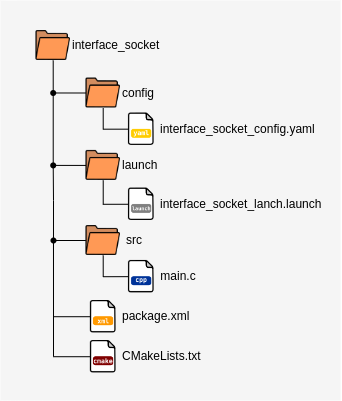
\includegraphics[scale=0.42]{imagens/rospackage.png}\\
		{\small \textbf{Fonte:} do autor}
    \end{center}\label{fig:clientdiretorios}
\end{figure}

A seguir será apresentada uma breve descrição de cada item do pacote:
 
\textbf{config/interface\underline{\hspace{.07in}}socket\underline{\hspace{.07in}}config.yaml:} Arquivo com o qual o usuário pode mudar alguns parâmetros de configuração da comunicação, como IP do servidor ou alguns outros parâmetros do tópico que será lido, como pode ser visto na Figura~\ref{fig:codigoconfig}. Essa mudança pode ocorrer sem a necessidade de recompilar o código fonte, o que pode dar flexibilidade ao usuário do pacote durante o desenvolvimento de uma nova aplicação, que poderá ser configurada sem alterações no código fonte do nó. 

\begin{figure}[ht]
\caption{Configurações do cliente}
\begin{center}
\begin{lstlisting}[language=C++, backgroundcolor=\color{gray!10}]
 server_ip: "127.0.0.1"
 port: 4242

 fps: 15
 encoding: "rgb8"
 height: 720
 width: 1280
 step: 3840
 header.frame_id: "camera_link"
\end{lstlisting}
{\small \textbf{Fonte:}Elaborado pelo autor}	
\end{center}\label{fig:codigoconfig}
\end{figure}
	

\textbf{launch/interface\underline{\hspace{.07in}}socket.launch:} Arquivo responsável chamar a execução do nó, além de carregar os parâmetros presentes no arquivo config.yaml no servidor de parâmetro do ROS\@.

\textbf{src/main.cpp:} Código fonte do executável, ou seja, o código fonte do nó presente neste pacote.

\textbf{package.xml:} Manifesto do pacote é o arquivo que define as propriedades do pacote, como por exemplo, nome do pacote, autor, e dependências. Deve estar presente em todos os pacotes ROS~\cite{RosPkgXml}.


\textbf{CmakeLists.txt:} Contém instruções e diretivas para configuração do processo de compilação do pacote.

O pacote cliente disponibiliza apenas um executável, ou seja, apenas um nó. Assim que o no é executado ele realiza a requisição para estabelecer a conexão com o servidor: com a conexão estabelecida o cliente pode dar início à sua função, ler dados de um tópico e enviá-los ao servidor. Antes de serem enviados ao servidor, os dados precisam ser preparados: informações importantes para o funcionamento interno do ROS, como campos dos cabeçalho, ou timestamp das mensagens, não serão enviados ao servidor. Ou seja, apenas os dados brutos são enviados, contribuindo para a diminuição de dados trafegando na rede. Na Figura~\ref{fig:codreaddata} podemos ver que não função de \textit{callback} do tópico de entrada do cliente, é retirada anas os dados da mensagem, carregando-os na variável que será enviada ao servidor.

\begin{figure}[ht]
\caption{Função Callback para o tópico lido pelo cliente}
\begin{center}
\begin{lstlisting}[language=C++, backgroundcolor=\color{gray!10}]
 // Variavel que armazena apenas os dados contidos no 
 // topico lido pleo cliente
 std::vector<uint8_t> dados_out(MSG_LEN);
 
 void image_rawCallback 
 		(const sensor_msgs::Image::ConstPtr & image){
 	// Apenas o campo data he armazenado na variavel
 	dados_out = image->data;
 }

\end{lstlisting}
{\small \textbf{Fonte:}Elaborado pelo autor}	
\end{center}\label{fig:codreaddata}
\end{figure}
		

Após os dados serem enviados ao servidor, o cliente deve ser capaz de recebê-los assim que o servidor atender à requisição. Neste ponto os dados já foram processados pelos circuitos do FPGA, mas como apenas os dados brutos foram enviados ao servidor, o cliente precisa montar novamente a mensagem, disponibilizando os dados processados a partir do tópico de saída, para que os outros nós do sistema possam utilizar esses dados em suas funcionalidades. O processo descrito anteriormente é relativamente simples, como pode ser visto no fluxograma simplificado da Figura~\ref{fig:clientfluxo}


\begin{figure}[ht]
	\caption{Fluxograma pacote cliente}
	\begin{center}
		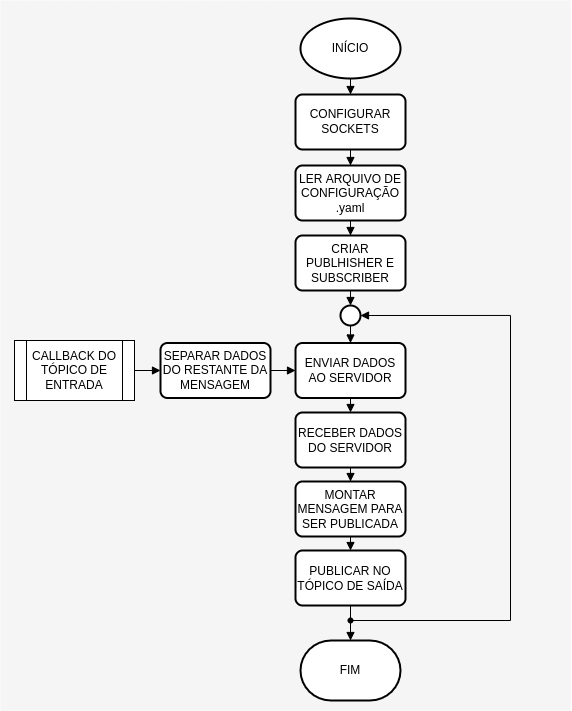
\includegraphics[scale=0.47]{imagens/fluxogramaCliente.png}\\
		{\small \textbf{Fonte:} do autor}
    \end{center}\label{fig:clientfluxo}
\end{figure}


\section{Outras alternativas}

Se seu objetivo for apenas estabelecer a comunicação entre dois dispositivos, já existe um pacote ROS pronto que atenderá a sua necessidade. O \textit{ROS serial} é uma pacote que tem como principal objetivo permitir a comunicação entre o ROS e outro dispositivo que possua uma porta serial ou uma interface de rede~\cite{RosSeria}. Sendo assim o ROS serial seria uma opção genérica, que não depende do dispositivo de hardware. Além do ROS serial, foi encontrado um trabalho em que os autores estabeleceram a comunicação entre o ROS e um FPGA\@. 

No trabalho de Yamashina et al. (2005), são demonstradas três técnicas para realizar a conexão entre o FPGA e o ROS, que se diferem da proposta por essa pesquisa. A escolha por desenvolver um novo pacote para executar a mesma função se fez necessário pela necessidade de alta taxa de transferência de dados entre o ROS e o SoC para que seja aceitável a utilização do SoC com a finalidade de acelerar o processamento por hardware. 

Desenvolvendo um novo pacote de comunicação podemos extrair o máximo de desempenho da rede, como por  exemplo, escolhendo o melhor protocolo (UDP ou TCP) e transferindo apenas os dados para o processamento da informação. Todos os códigos do cliente podem ser encontrados no repositório disponível em~\cite{interface-socket}.

\chapter{Servidor}

% Introdução ao programa servidor
%=====================================
O servidor é o software embarcado no HPS do Soc. Ele é o responsável por gerenciar a comunicação entre a interface de rede por onde recebe os dados provenientes do pacote ROS (cliente) e o FPGA\@. A primeira etapa a ser concluída no desenvolvimento do servidor é compilação de uma versão linux para processadores ARM que será instalada no kit de desenvolvimento. O fluxo de boot do linux na placa é resumido na Figura~\ref{fig:linux}. 

% explicar processo de boot
%=====================================
\section{Processo de BOOT}
O primeiro elemento de software é o \textit{Boot ROM} que está gravado de fábrica internamente no dispositivo. Os arquivos de \textit{PreLoader},\textit{ U-boot} e do sistemas de aquivos do linux são salvos em um cartão de memória micro SD\@. O \textit{Secondary Program Loader - SPL}, conhecido como \textit{PreLoader}, é executado a partir da Boot ROM\@. Ele é responsável por configurar o sistema para que o \textit{bootloader} (U-boot) possa ser executado. A Intel fornece uma ferramenta chamada BSP editor que, a partir de arquivos que descrevem o hardware, podem gerar o PreLoader para o projeto específico~\cite{SocLinux}.  

\begin{figure}[ht]
	\caption{Boot linux embarcado}
	\begin{center}
		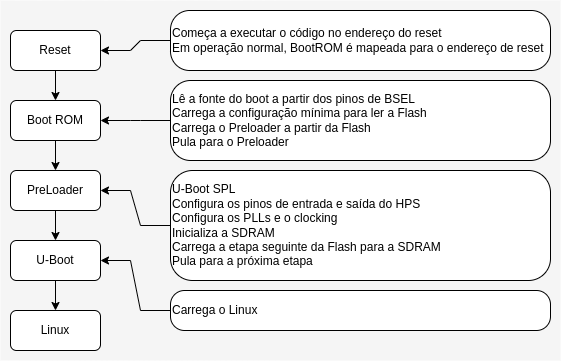
\includegraphics[scale=0.7]{imagens/embeddedLinux.png}\\
		{\small \textbf{Fonte:}\cite{SocLinux}}
    \end{center}\label{fig:linux}
\end{figure}

A etapa seguinte ao \textit{PreLoader} é o \textit{bootloader}. Nessa fase do boot todas as questões de baixo nível do SoC, como por exemplo, os clocks, pinos e SDRAM, já foram inicializados e estão prontos. O objetivo do bootloader, é obter essas informações do sistema e fazer com que ele funcione até o ponto onde o linux possa ser iniciado. Outra função importante do U-boot em um SoC Intel é programar o FPGA~\cite{SocLinux}.

% Explicar a distribuição usada
%=====================================
\section{Distribuição Linux rsyocto}
Com todos os arquivos necessários para o boot do sitema já gerados a partir das ferramentas de desenvolvimento da Intel, poderemos escolher nosso sistema operacional. O sistema escolhido foi uma distribuição linux desenvolvida exclusivamente para SoCs da Intel com fpga integrado, como pode ser observado na descrição da distribuição disponível em~\cite{rsyocto}:

\begin{citacao}
	``\textbf{rsyocto} is an open source Embedded Linux Distribution designed with the Yocto Project and with a custom build flow to be optimized for Intel SoC-FPGAs (Intel Cyclone V and Intel Arria 10 SX SoC-FPGA with an ARM Cortex-A9) to achieve the best customization for the strong requirements of modern embedded SoC-FPGA applications.''
\end{citacao} 

\begin{figure}[ht]
	\caption{Overview do rsyocto}
	\begin{center}
		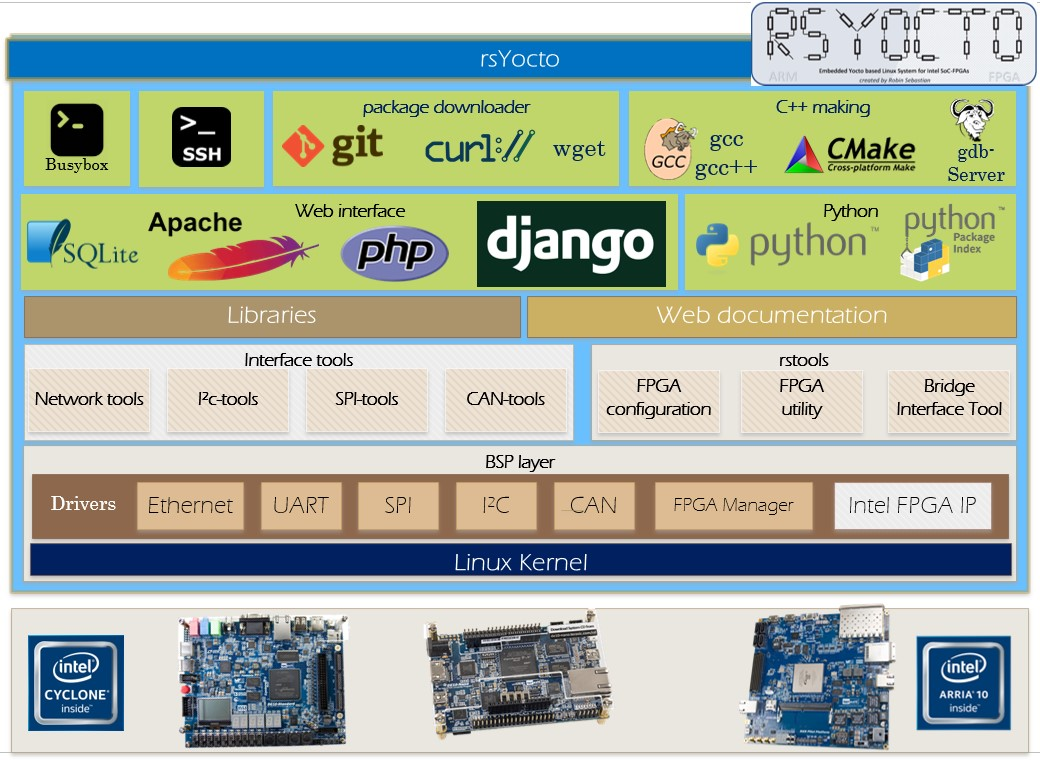
\includegraphics[scale=0.45]{imagens/rsYoctoLayers.jpg}\\
		{\small \textbf{Fonte:}\cite{rsyocto}}
    \end{center}\label{fig:rsyocto}
\end{figure}

% Explicar o códgo do servidor
%=====================================
\section{Interface socket server}
Com o linux já devidamente configurado, ele já pode ser inicializado no processador do SoC, assim podemos iniciar o desenvolvimento do servidor. No primeiro momento devemos realizar o download do código fonte da biblioteca de comunicação, a libinterfacesocket, que já foi detalhada anteriormente, o código fonte pode ser baixado em~\cite{interface-socket-server}. Com os arquivos já no sistema de diretórios do SoC devemos realizar a compilação e a instalação da libinterfacesocket, só assim o servidor terá acesso a suas funcionalidades. 

O acesso do servidor ao FPGA é feito através de mapeamento de endereços do linux, os SoCs Intel possuem uma arquitetura de memória mapeada. Desta forma, além da biblioteca desenvolvida durante a pesquisa, um outro arquivo cabeçalho é necessário para facilitar o acesso aos endereços de memória do HPS\@. Quando uma instância do processador ARM é incluída no projeto do QSys Designer, é gerado um arquivo.sopcinfo no momento em que o projeto é compilado. Podemos usar esse arquivo como entrada da ferramenta \textit{sopc-create-header-files} presente no SoC EDS para gerar um novo arquivo com extensão \textit{.h}, que lista os endereços base de todos os módulos (IP) incluídos no FPGA\@. Portanto, o arquivo cabeçalho gerado disponibiliza o \textit{offset} do endereço em que cada periférico está localizado para cada uma das FPGA-bridges disponíveis. Deste modo o servidor pode enviar ou receber dados ao periférico conhecendo o endereço da FPGA-bridge em que este periférico está conectado e o seu nome, sem a necessidade de se conhecer exatamente o seu endereço.

O Servidor mantém porta aberta para estabelecer uma conexão com o cliente e assim que a conexão é estabelecida, o cliente já pode começar a enviar os dados. Ao receber os dados do cliente, o servidor envia-os ao FPGA que os processa e os devolve ao servidor para que ele possa reenviar os dados já processados ao cliente. Um fluxograma simplificado desse processo pode ser visualizado na Figura \ref{fig:fluxoServidor}.

\begin{figure}[ht]
	\caption{Fluxograma simplificado do servidor}
	\begin{center}
		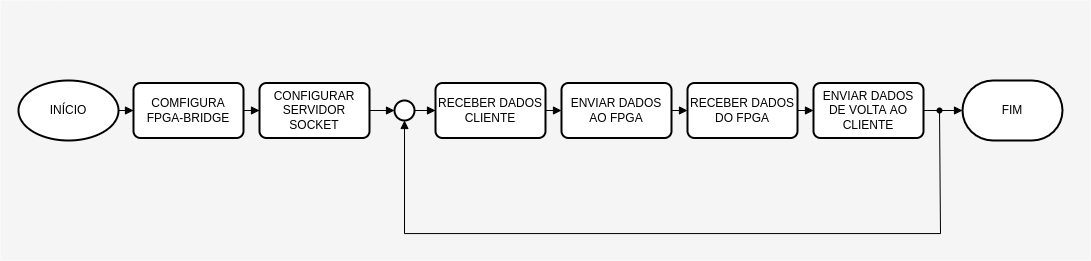
\includegraphics[scale=0.47]{imagens/fluxogramaServidor.png}\\
		{\small \textbf{Fonte:}Elaborado pelo autor}
    \end{center}\label{fig:fluxoServidor}
\end{figure} 


\part{Resultados}
\chapter{Resultados Alcançados}\label{cap:result}

Para validar a comunicação foram idealizados dois ensaios: o primeiro com o objetivo de testar o fluxo completo de troca de dados entre um nó ROS e uma aplicação embarcada no FPGA; o segundo ensaio teve o objetivo de testar um fluxo grande de dados trafegando entre o ROS e o SoC.

O objetivo do primeiro ensaio era verificar a comunicação completa entre o nó ROS e um IP sendo executado no FPGA. Para isso,  foi projetado um circuito simples que calcula o dobro de um número,  este circuito foi instanciado no FPGA, a \textit{HPS-to-FPGA Lightweight} bridge foi utilizada para realizar a comunicação entre o servidor, rodando no HPS, e o FPGA. No nó cliente, rodando no ROS, foram configurados dois tópicos, um para o número a ser enviado e outro para receber o resultado calculado pelo FPGA, da mesma maneira que mostra o esquema da Figura \ref{fig:arquitetura}. A comunicação foi estabelecida e o sistema se comportou como esperado.

O segundo ensaio tinha a intenção de testar a sobrecarga de dados na rede e avaliar o comportamento da mesma. Neste teste foi realizado o envio de uma \textit{stream} de vídeo com resolução de 1280x720 em 15 fps capturada a partir de uma webcam dentro do ambiente ROS, ou seja, um nó ROS acessa a webcam e disponibiliza a \textit{stream} de vídeo em um tópico sendo publicado e uma frequência de 15Hz. A partir deste ensaio foi possível realizar a estimativa de largura de banda utilizada e o \textit{delay} gerado na comunicação. No gráfico da Figura~\ref{fig:speed} podemos ver a velocidade da comunicação, em bits por segundo, em função do tempo de transmissão. As velocidades alcançadas superaram a barreira dos 400 Mbps.

\begin{figure}[ht]
	\caption{Gráfico velocidade de transmissão}
	\begin{center}
		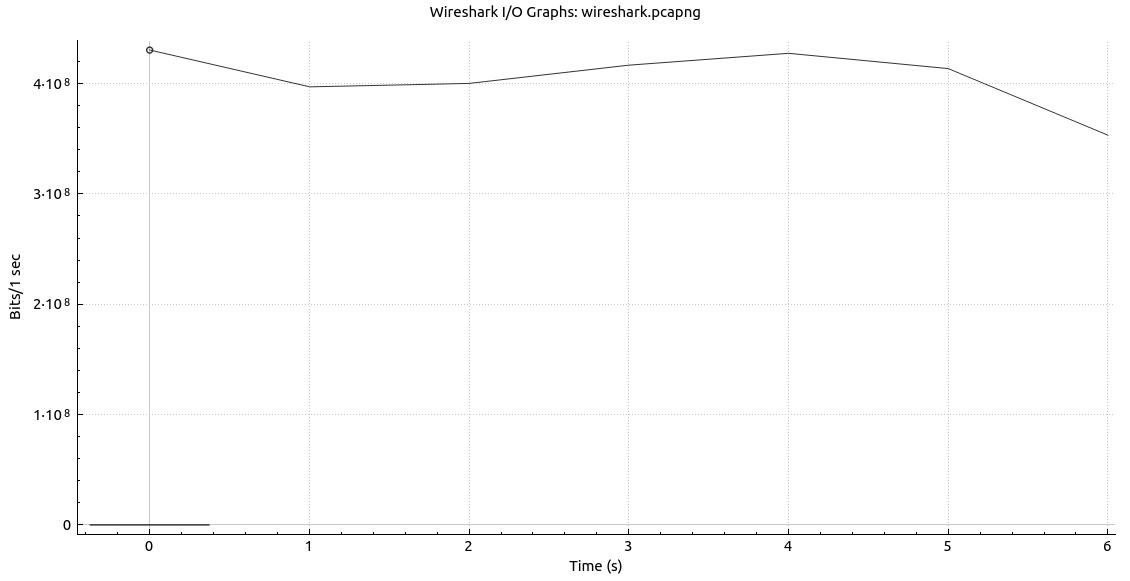
\includegraphics[scale=0.42]{imagens/speed.jpg}\\
		{\small \textbf{Fonte:} Elaborado pelo autor}
    \end{center}\label{fig:speed}
\end{figure}

Os atrasos gerados podem ser vistos na Figura~\ref{fig:delay}, onde é possível observar o \textit{Round Trip Time} (RTT), que é o atraso total de um pacote TCP, ou seja, o tempo que um pacote leva para ir da origem ao destino e retornar à origem. Os atrasos máximos ficaram por volta de 10ms. 

\begin{figure}[ht]
	\caption{Atrasos gerados durante a comunicação}
	\begin{center}
		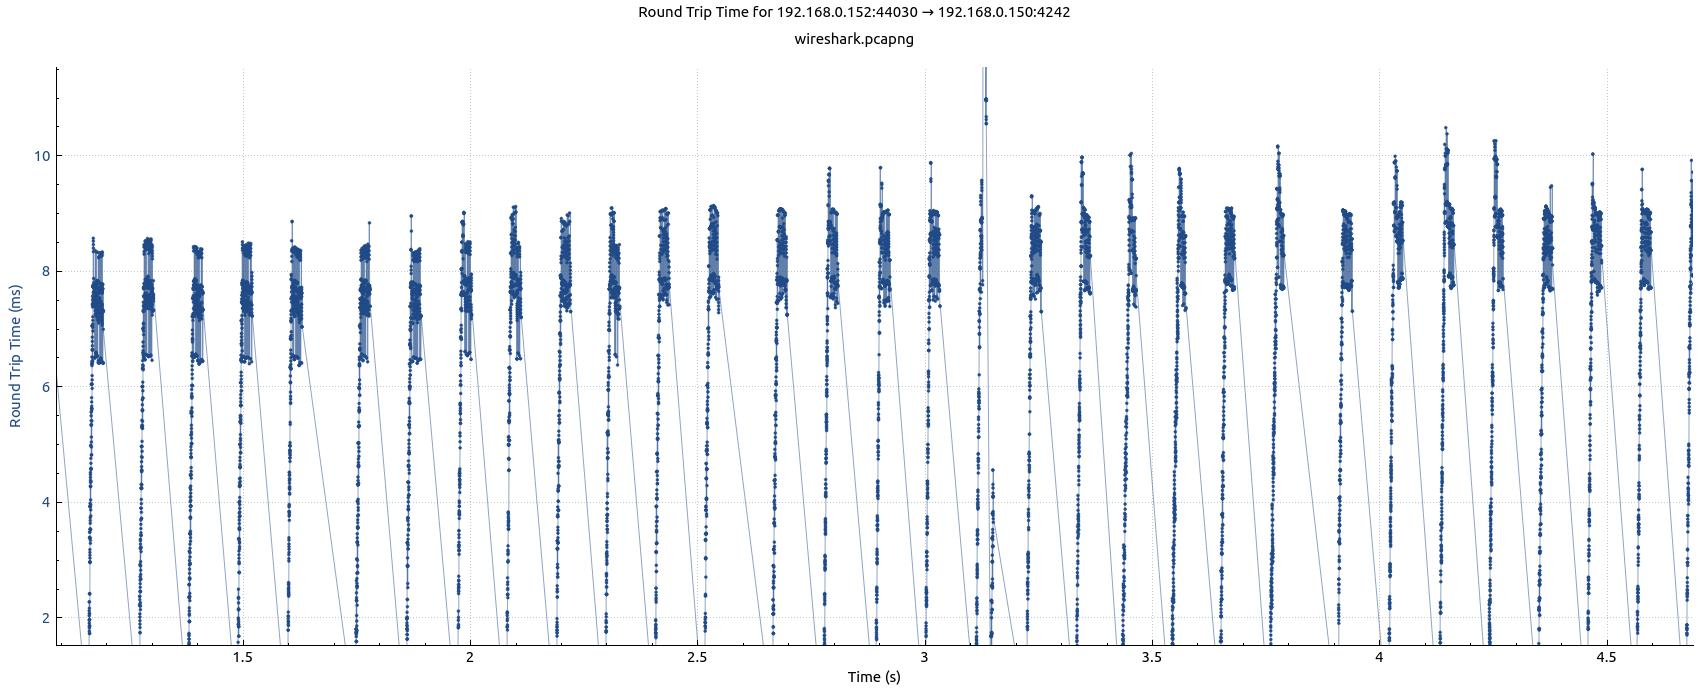
\includegraphics[scale=0.35]{imagens/delay.jpg}\\
		{\small \textbf{Fonte:} Elaborado pelo autor}
    \end{center}\label{fig:delay}
\end{figure}

% ---
% Conclusão
% ---
\chapter{Estudos futuros}
% ---

Capítulo conclusão
\chapter{Estudos futuros}\label{cap:trabfut}

Por se tratar de um trabalho interdisciplinar que abrange áreas como programação de rede, compilação e configuração de linux embarcado, desenvolvimento com o ROS e com SoC, trabalhos futuros podem dar ênfase a alguma dessas áreas específicas, otimizando alguns pontos do projeto para se alcançar maiores taxas de transferência, tornar o sistema ainda mais genérico e fácil de ser usados por outros grupos de trabalho que tenham o interesse de adicionar processamento por hardware em seus projetos de robótica. Como por exemplo, os métodos disponibilizados pela biblioteca de comunicação podem oferecer versões que façam uso do protocolo UDP, o que poderia diminuir consideravelmente o delay observador durante os ensaios. 
 

% Adiciona espaço de parte no Sumário
\phantompart%
%-------------------------------------------------------------------------------------
%		CONTEÚDO PÓS-TEXTUAL
%		Parte do documento que aparece após o capítulo de conclusão, incluindo 
%		bibliografia e anexos.
%-------------------------------------------------------------------------------------
\postextual\bibliography{references} 

%\glossary

% Apendices
%-------------------------------
% \begin{apendicesenv}
% \partapendices
% % ----------------------------------------------------------
\chapter{Quisque libero justo}
% ----------------------------------------------------------

\lipsum[50]

% ----------------------------------------------------------
\chapter{Nullam elementum urna vel imperdiet sodales elit ipsum pharetra ligula
ac pretium ante justo a nulla curabitur tristique arcu eu metus}
% ----------------------------------------------------------
\lipsum[55-57]
% \end{apendicesenv}

% Anexos
%-------------------------------
% \begin{anexosenv}
% \partanexos
% % ---
\chapter{Morbi ultrices rutrum lorem.}
% ---
\lipsum[30]
% % ---
\chapter{Cras non urna sed feugiat cum sociis natoque penatibus et magnis dis
parturient montes nascetur ridiculus mus}
% ---

\lipsum[31]
% 
% ---
\chapter{Fusce facilisis lacinia dui}
% ---

\lipsum[32]
% \end{anexosenv}

% Indice remissivo
%-------------------------------
% \phantompart
% \printindex

\end{document}
